\documentclass[12pt, a4paper]{article}

\usepackage[utf8]{inputenc}
\usepackage[spanish]{babel}
\usepackage{amsmath, amssymb, amsfonts}
\usepackage{graphicx}
\usepackage{geometry}
\usepackage{hyperref}
\usepackage{booktabs}
\usepackage{xcolor}
\usepackage{subcaption} % Añadido para agrupar gráficas

\geometry{top=2.5cm, bottom=2.5cm, left=2.5cm, right=2.5cm}

\title{\vspace{-2cm}\textbf{Primer Parcial: Optimización y Paralelización en Dinámica Cuántica}\\
\large Sistemas Distribuidos - Computación de Alto Desempeño}
\author{
    Camilo Huertas \quad Sebastian Rodriguez \\[0.3cm]
    \small Proyecto Curricular de Física \\
    \small Universidad Distrital Francisco José de Caldas
}
\date{\today}

\begin{document}

\maketitle

\begin{abstract}
El presente informe detalla el rediseño, optimización y paralelización de la solución numérica de la ecuación de Schrödinger dependiente del tiempo para un paquete de ondas gaussiano. Se parte de dos implementaciones base (Pseudo-espectral y aproximación de Cayley) y se proponen dos métodos adicionales (Expansión de Chebyshev y subespacios de Krylov-Lanczos). Se evalúa el impacto de la jerarquía de memoria mediante optimización serial y banderas de compilación, culminando con una paralelización en memoria compartida vía OpenMP.
\end{abstract}

\section{Descripción del Problema Físico}
El problema central abordado en este trabajo consiste en la simulación de la dinámica cuántica de una partícula no relativista mediante la solución numérica de la ecuación de Schrödinger dependiente del tiempo en una dimensión:
$$ i \frac{\partial \psi(x,t)}{\partial t} = \hat{H} \psi(x,t) $$
donde se ha asumido un sistema de unidades atómicas ($\hbar = 1$) y $\hat{H}$ representa el operador Hamiltoniano, compuesto por los términos de energía cinética y potencial:
$$ \hat{H} = -\frac{1}{2m}\frac{\partial^2}{\partial x^2} + V(x) $$
La dinámica del sistema se estudia evaluando la evolución temporal de un estado inicial $\psi(x,0)$, el cual se modela mediante un paquete de ondas gaussiano. Este enfoque permite analizar la propagación y dispersión del paquete al interactuar con diferentes perfiles de potencial $V(x)$. 

Desde la perspectiva de la física computacional, el desafío radica en aplicar el operador de evolución temporal $\hat{U}(t) = e^{-i\hat{H}t}$ de manera discreta. Para que la solución numérica sea físicamente rigurosa, el método seleccionado debe ser estrictamente unitario, garantizando así la conservación de la probabilidad ($\int |\psi(x,t)|^2 dx = 1$) en cada paso de tiempo computado.


\section{Justificación de los Métodos Numéricos}
La selección de los esquemas numéricos para integrar la ecuación de Schrödinger dependiente del tiempo es fundamental, dado que distintas formulaciones conducen a estructuras computacionales que impactan directamente el rendimiento y uso de caché. A continuación, se justifican los métodos seleccionados bajo criterios físicos, matemáticos y de complejidad algorítmica.

\subsection{Método 1 (Base): Pseudo-Espectral (Split-Operator con FFT)}
Este método separa el operador de evolución en sus componentes de energía cinética ($\hat{K}$) y potencial ($\hat{V}$). Utiliza la Transformada Rápida de Fourier (FFT) para evaluar la acción del operador cinético en el espacio de momentos, aplicando la aproximación:
$$ \psi(x, t+\Delta t) \approx e^{-i \hat{V} \Delta t / 2} \mathcal{F}^{-1} \left\{ e^{-i \hat{K} \Delta t} \mathcal{F} \{ \psi(x,t) \} \right\} e^{-i \hat{V} \Delta t / 2} $$
\begin{itemize}
    \item \textbf{Estabilidad y Convergencia:} Es incondicionalmente estable y estrictamente unitario (conserva la norma de la función de onda). Presenta convergencia espectral (el error espacial decae exponencialmente).
    \item \textbf{Complejidad Algorítmica:} Dominada por la FFT, escalando como $\mathcal{O}(N \log N)$, donde $N$ es el tamaño de la malla espacial. Computacionalmente, sufre de baja localidad espacial debido a los saltos de memoria requeridos por la FFT.
\end{itemize}

\subsection{Método 2 (Base): Aproximación de Cayley}
Este método emplea la transformada de Cayley para aproximar el operador de evolución temporal, lo que resulta en un esquema implícito de diferencias finitas análogo al método de Crank-Nicolson:
$$ e^{-i\hat{H}\Delta t} \approx \frac{1 - i\hat{H}\Delta t / 2}{1 + i\hat{H}\Delta t / 2} $$
Computacionalmente, esto requiere resolver un sistema lineal tridiagonal algebraico en cada paso de tiempo:
$$ \left(1 + i \frac{\Delta t}{2} \hat{H}\right) \psi(x, t+\Delta t) = \left(1 - i \frac{\Delta t}{2} \hat{H}\right) \psi(x,t) $$
\begin{itemize}
    \item \textbf{Estabilidad y Convergencia:} Es estrictamente unitario e incondicionalmente estable. El error de truncamiento temporal es de segundo orden $\mathcal{O}(\Delta t^2)$.
    \item \textbf{Complejidad Algorítmica:} Escala linealmente $\mathcal{O}(N)$ gracias al uso de algoritmos eficientes para matrices tridiagonales (como el algoritmo de Thomas). Sin embargo, la naturaleza implícita del sistema introduce fuertes dependencias algorítmicas de datos que limitan severamente su paralelización.
\end{itemize}

\subsection{Método Propuesto A: Expansión Polinomial de Chebyshev}
Sustituye la aproximación de diferencias finitas temporales expandiendo el operador de evolución unitaria en una base de polinomios de Chebyshev complejos. Discretizando espacialmente el Hamiltoniano normalizado $\hat{H}_{norm}$, la acción sobre la función de onda se evalúa como:
$$ \psi(x, t+\Delta t) \approx e^{-i E_{avg} \Delta t} \sum_{k=0}^{M} c_k \phi_k(x) $$
donde los coeficientes dependen de las funciones de Bessel de primera especie $c_k = 2(-i)^k J_k(\alpha)$, y $\phi_k$ se obtienen mediante una relación de recurrencia tridiagonal.
\begin{itemize}
    \item \textbf{Estabilidad y Convergencia:} Altamente estable siempre que el espectro del Hamiltoniano sea correctamente normalizado al intervalo $[-1, 1]$. El error temporal converge exponencialmente.
    \item \textbf{Complejidad Algorítmica:} Escala como $\mathcal{O}(M \cdot N)$, donde $M$ es el orden de expansión. Al usar diferencias finitas para la acción de $\hat{H}$, los accesos a memoria son puramente locales, ideal para optimización de caché y vectorización SIMD.
\end{itemize}

\subsection{Método Propuesto B: Subespacios de Krylov (Método de Lanczos)}
Este método construye una base ortonormal reducida (espacio de Krylov) de dimensión $m$ adaptada al estado instantáneo de la función de onda. El Hamiltoniano global se proyecta y tridiagonaliza en este subespacio reducido ($T_m = V_m^\dagger \hat{H} V_m$), aproximando la evolución como:
$$ \psi(x, t+\Delta t) \approx V_m e^{-i T_m \Delta t} V_m^\dagger \psi(x,t) $$
\begin{itemize}
    \item \textbf{Estabilidad y Convergencia:} Es un método fuertemente unitario y altamente estable. La aproximación de la propagación es casi exacta dentro del subespacio generado.
    \item \textbf{Complejidad Algorítmica:} Requiere $m$ aplicaciones del Hamiltoniano, escalando como $\mathcal{O}(m \cdot N)$. La diagonalización de la matriz reducida es $\mathcal{O}(m^3)$, un costo despreciable ya que típicamente $m \ll N$. Se beneficia enormemente de operaciones densas de álgebra lineal tipo BLAS.
\end{itemize}


\section{Análisis de Optimización Serial}
\label{sec:opt_serial}

Como parte del rediseño computacional, se llevó a cabo un proceso sistemático de optimización del código serial en sus diferentes implementaciones. Este análisis consistió en evaluar el impacto de las banderas de compilación \texttt{-O0}, \texttt{-O1}, \texttt{-O2} y \texttt{-O3}, así como la reorganización interna del algoritmo (optimización de bucles y localidad espacial) para mejorar el uso de la memoria caché. Las pruebas se ejecutaron en un procesador AMD Ryzen Threadripper 3990X (64 núcleos, 128 hilos) con 256 MiB de caché L3 y 2 MiB de caché L1D.

\subsection{Impacto de las Banderas de Compilación}

La optimización a nivel de compilador permite aprovechar características de hardware específicas sin alterar el código fuente. Se midieron los tiempos totales de ejecución variando el nivel de agresividad del compilador. Los resultados consolidados para las implementaciones base y propuestas se presentan en el Cuadro \ref{tab:banderas_compilacion}.

\begin{table}[h]
\centering
\caption{Tiempo de ejecución promedio (en segundos) según bandera de compilación y versión del código para los cuatro métodos numéricos.}
\label{tab:banderas_compilacion}
\resizebox{\textwidth}{!}{
\begin{tabular}{llcccc}
\toprule
\textbf{Método} & \textbf{Versión del Código} & \textbf{-O0 (s)} & \textbf{-O1 (s)} & \textbf{-O2 (s)} & \textbf{-O3 (s)} \\
\midrule
\textbf{1. Pseudo-espectral (FFT)} & Original & 1.946 & 1.886 & 2.081 & 2.996 \\
                                   & Optimizado (Tiling) & 2.264 & 0.643 & 0.661 & 0.706 \\
\midrule
\textbf{2. Cayley}                 & Original & 0.234 & 0.140 & 0.141 & 0.134 \\
                                   & Optimizado & 0.234 & 0.141 & 0.140 & 0.134 \\
\midrule
\textbf{3. Chebyshev}              & Original & 10.172 & 4.305 & 4.135 & 4.065 \\
                                   & Caché (Localidad) & 10.333 & 3.777 & 3.858 & 4.278 \\
\midrule
\textbf{4. Krylov-Lanczos}         & Original & 3.475 & 1.450 & 1.381 & 1.142 \\
                                   & Optimizado & 4.054 & 1.379 & 1.391 & 1.165 \\
\bottomrule
\end{tabular}}
\end{table}

De los resultados expuestos, se destaca el comportamiento en el \textbf{Método 1 (Pseudo-espectral)}. La versión original presenta anomalías con \texttt{-O3}, incrementando el tiempo de ejecución (hasta 2.99s), lo cual es típico cuando el compilador fuerza un desenrollado de bucles (\textit{loop unrolling}) y vectorizaciones en estructuras de datos con saltos de memoria inconsistentes (como los de la FFT), saturando la caché de instrucciones o registros. Sin embargo, al aplicar reestructuración espacial (versión \textit{Optimizada}), las banderas \texttt{-O1} a \texttt{-O3} reducen drásticamente el tiempo (de 2.26s a 0.64s), demostrando una sinergia exitosa entre la reestructuración manual del código y la automatización del compilador.

En los \textbf{Métodos 3 (Chebyshev) y 4 (Krylov-Lanczos)}, el escalamiento de rendimiento es claro y directo. Pasar de no optimizar (\texttt{-O0}) a niveles superiores reduce el tiempo a menos de la mitad (e.g., de 10.3s a 3.7s en Chebyshev). Esto indica un fuerte aprovechamiento del mapeo de variables en registros (evitando lecturas en RAM) y una eficiente vectorización SIMD en los cálculos densos y locales inherentes a las diferencias finitas y al álgebra matricial.

El impacto visual de estas reducciones de tiempo se puede apreciar en la Figura \ref{fig:barras_optimizacion}.

\begin{figure}[htbp]
    \centering
    \begin{subfigure}[b]{0.45\textwidth}
        \centering
        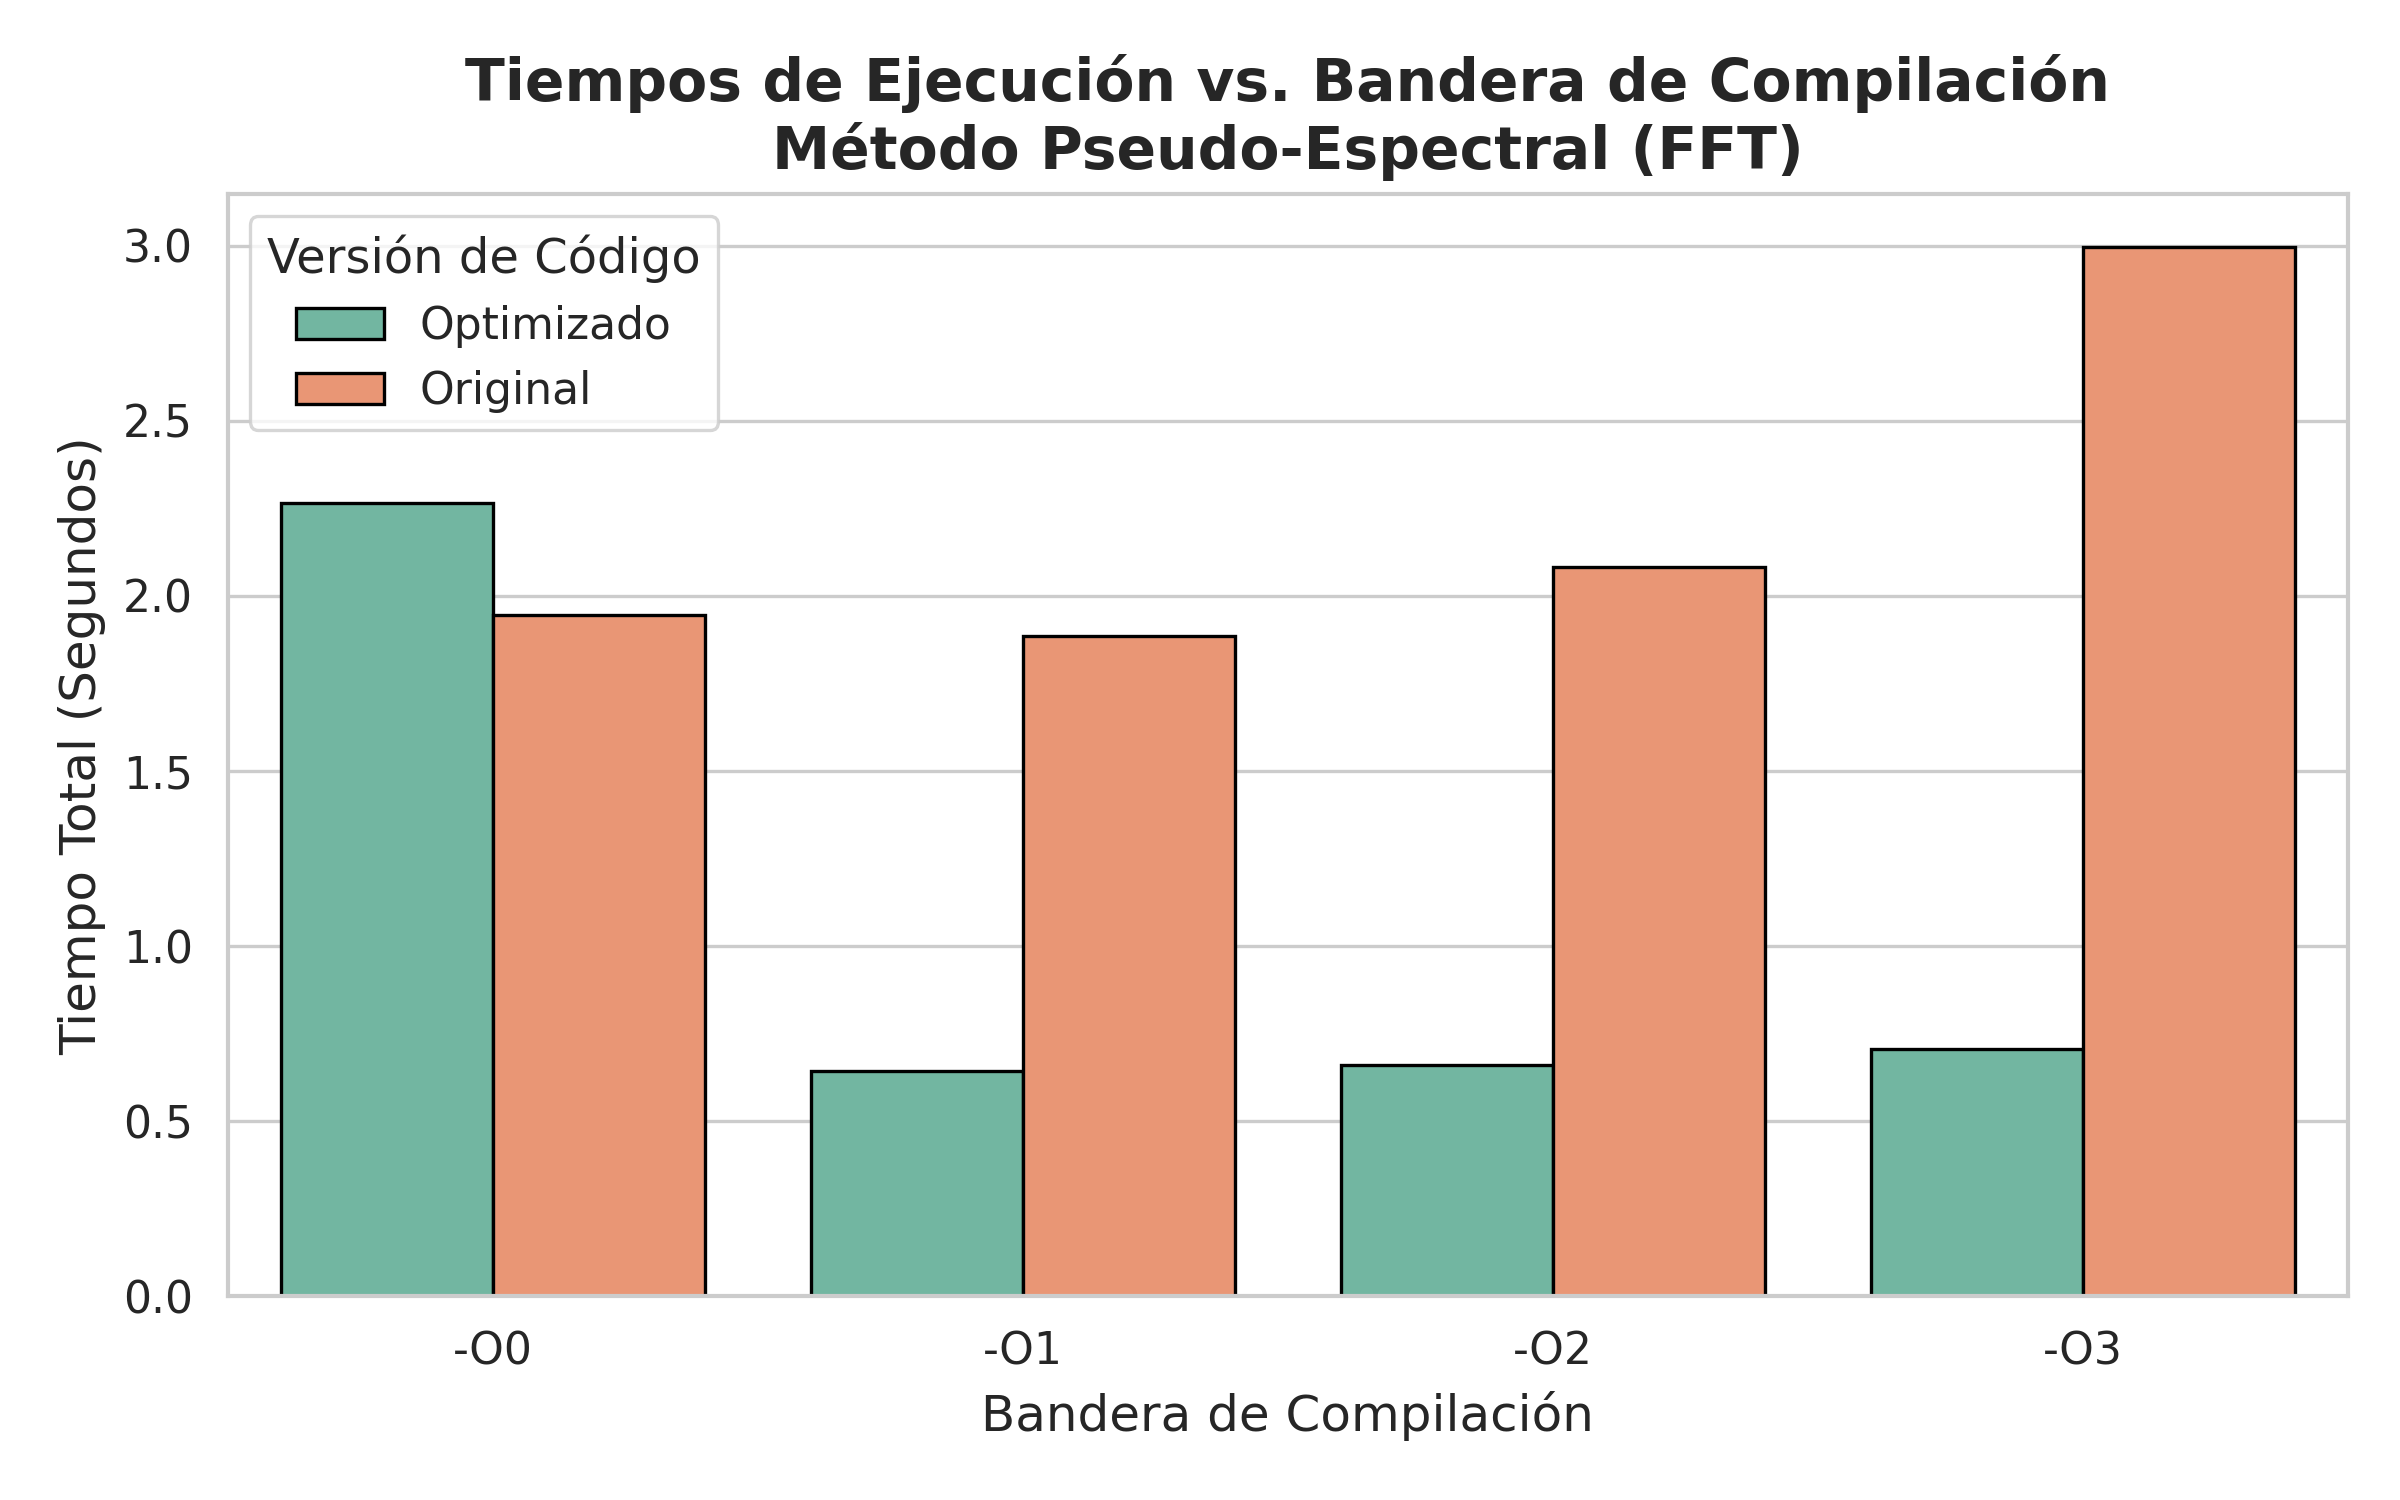
\includegraphics[width=\textwidth]{../../img/barras_optimizacion_code1.png}
        \caption{Método 1: Pseudo-Espectral (FFT)}
        \label{fig:opt_c1}
    \end{subfigure}
    \hfill
    \begin{subfigure}[b]{0.45\textwidth}
        \centering
        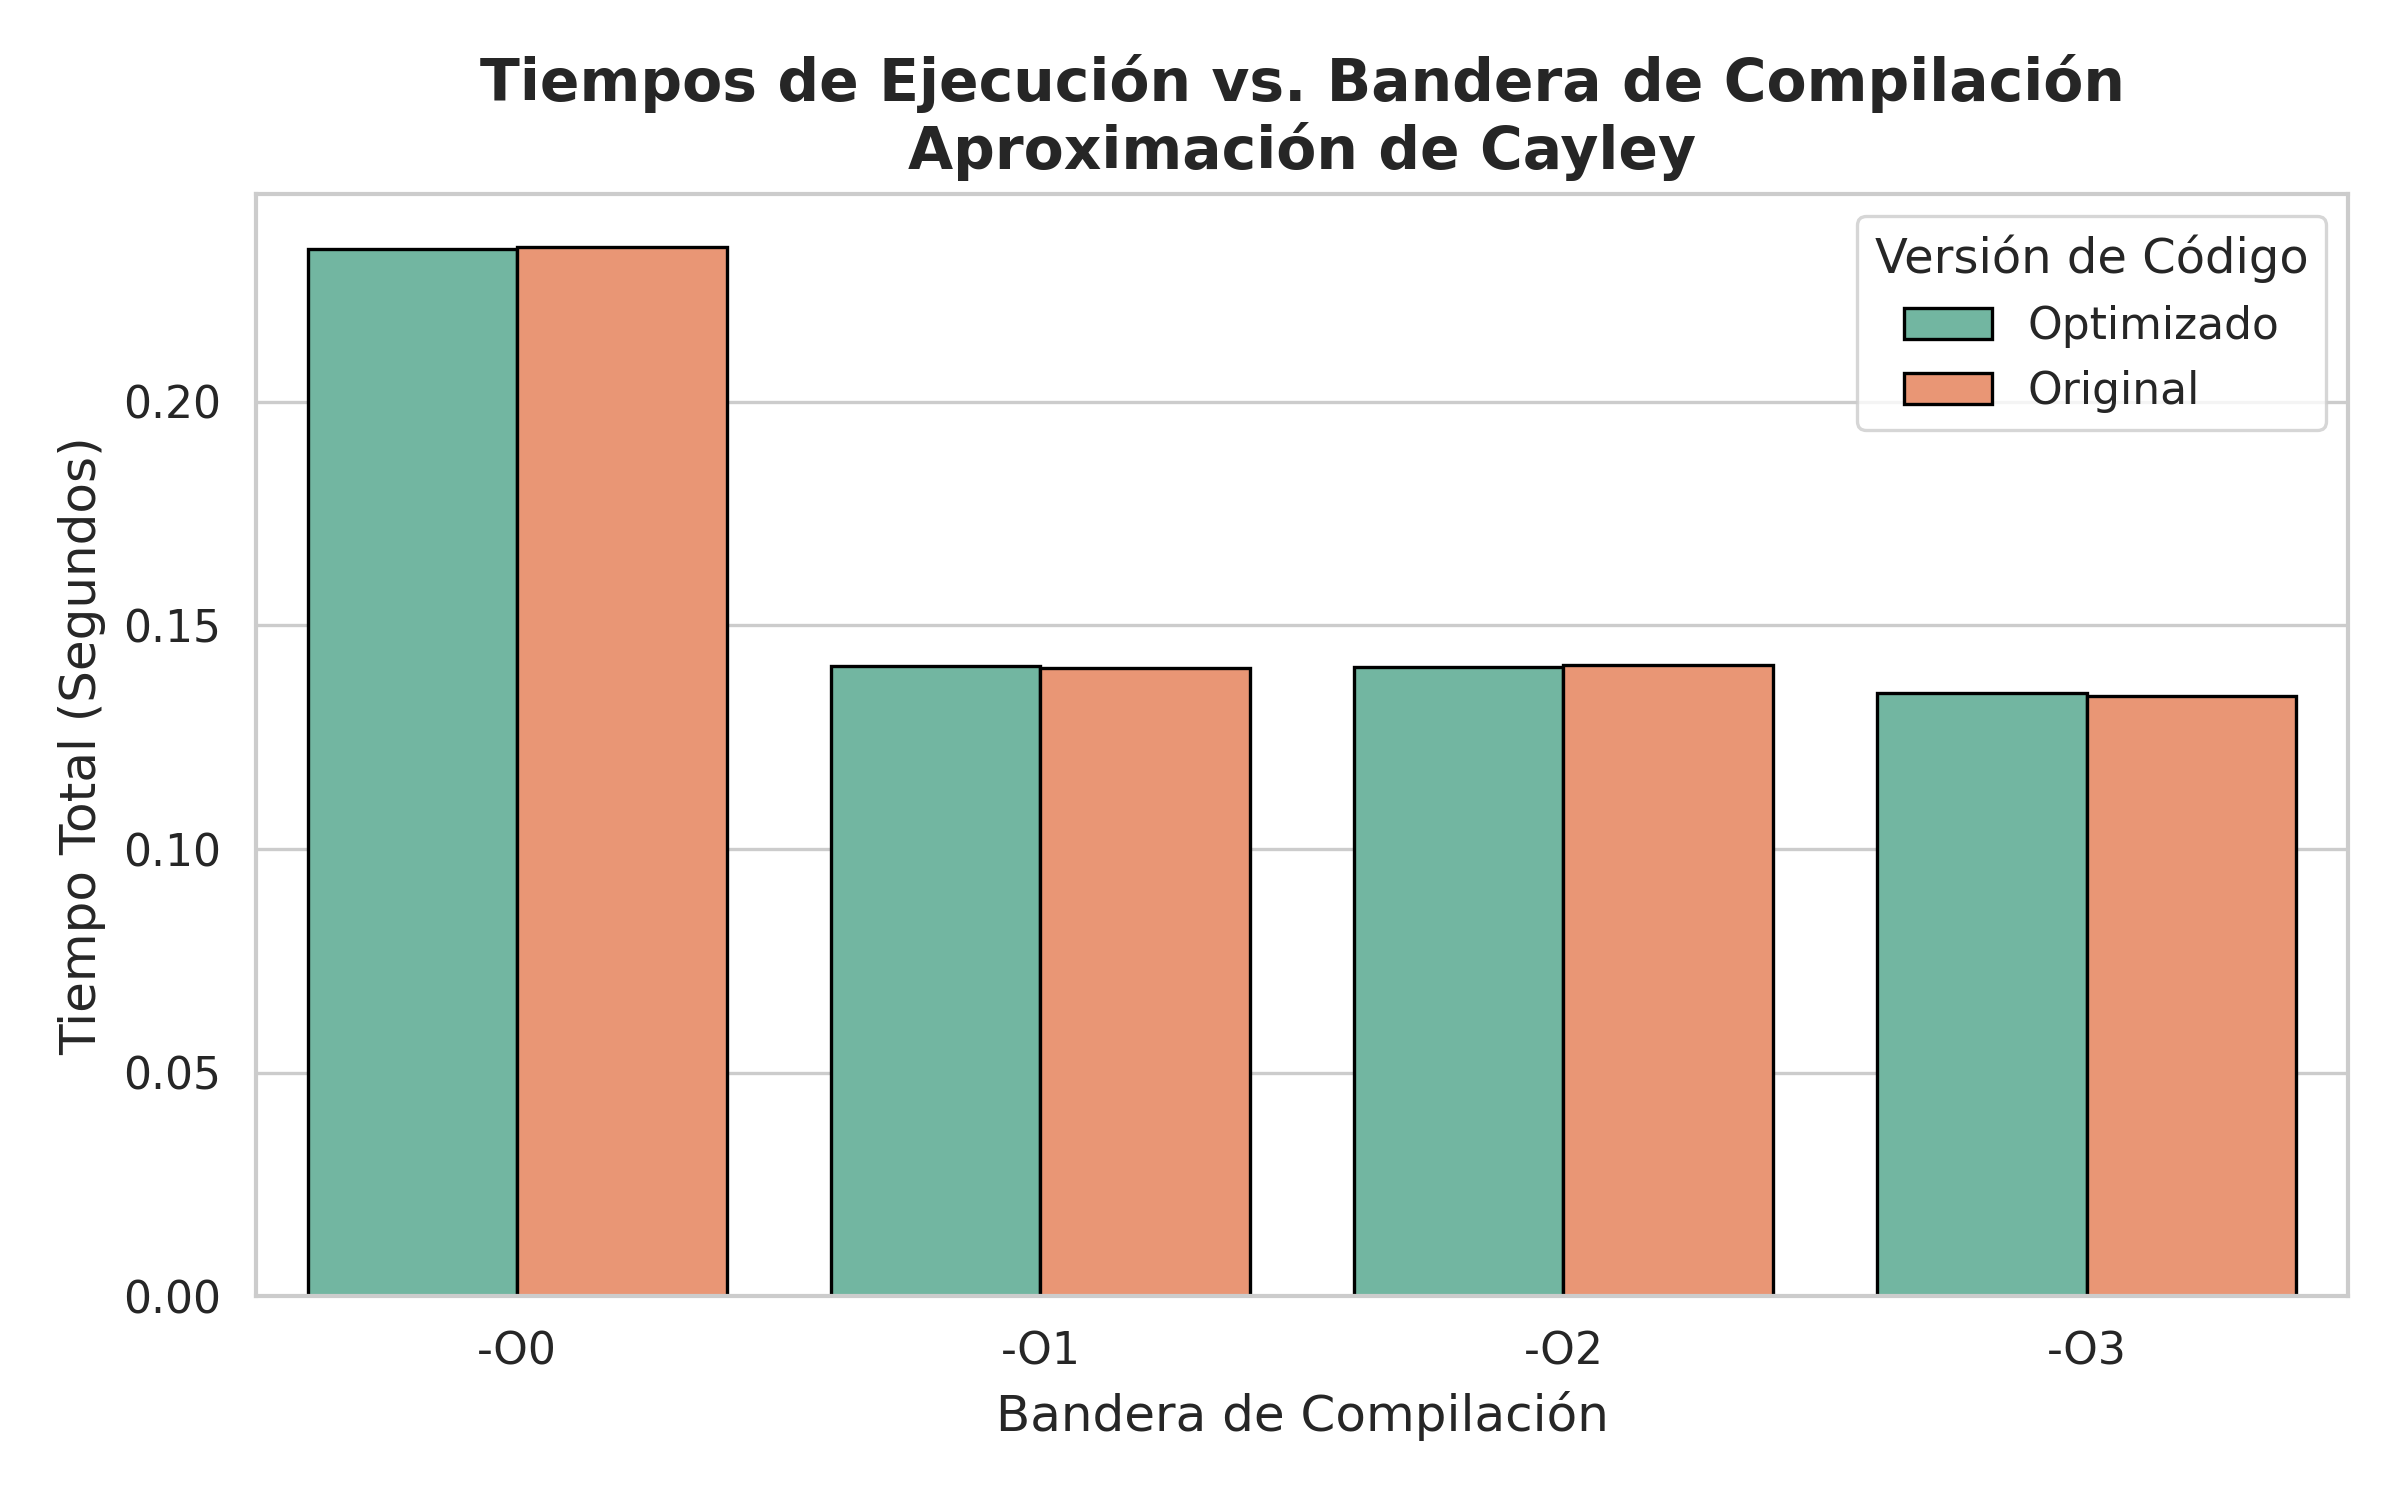
\includegraphics[width=\textwidth]{../../img/barras_optimizacion_code2.png}
        \caption{Método 2: Aproximación de Cayley}
        \label{fig:opt_c2}
    \end{subfigure}
    \vspace{0.5cm} % Espacio vertical entre las filas
    
    \begin{subfigure}[b]{0.45\textwidth}
        \centering
        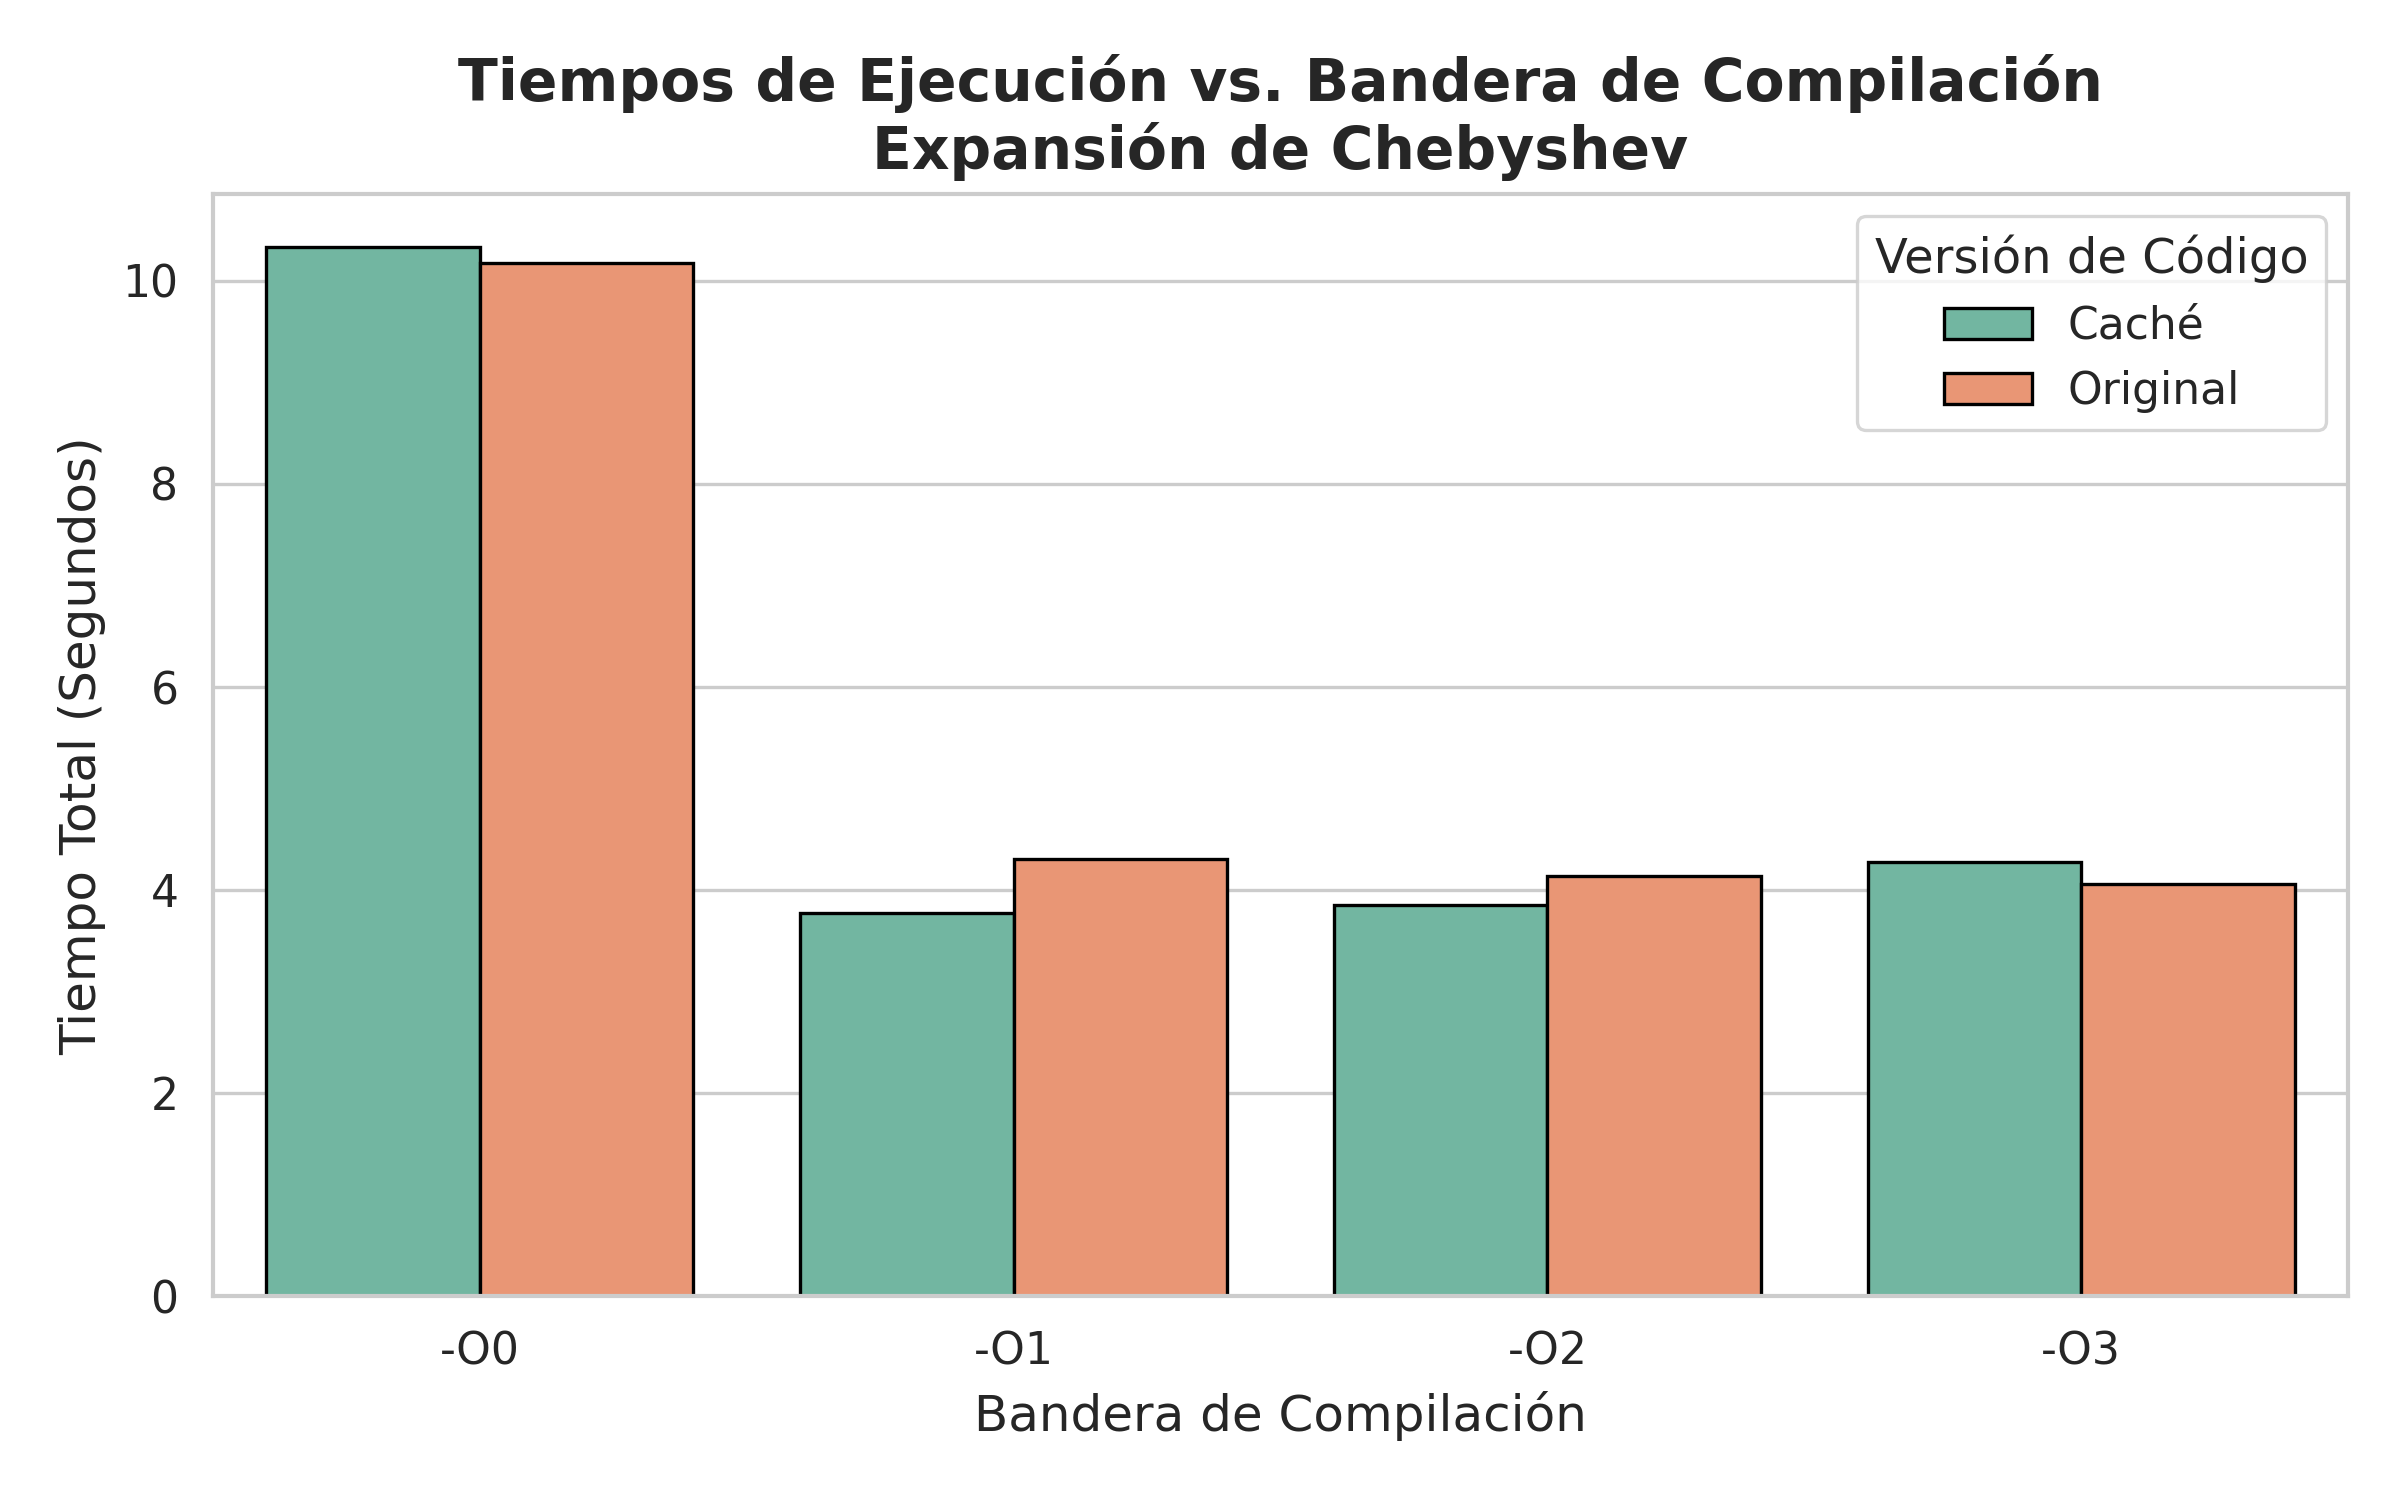
\includegraphics[width=\textwidth]{../../img/barras_optimizacion_code3.png}
        \caption{Método 3: Expansión de Chebyshev}
        \label{fig:opt_c3}
    \end{subfigure}
    \hfill
    \begin{subfigure}[b]{0.45\textwidth}
        \centering
        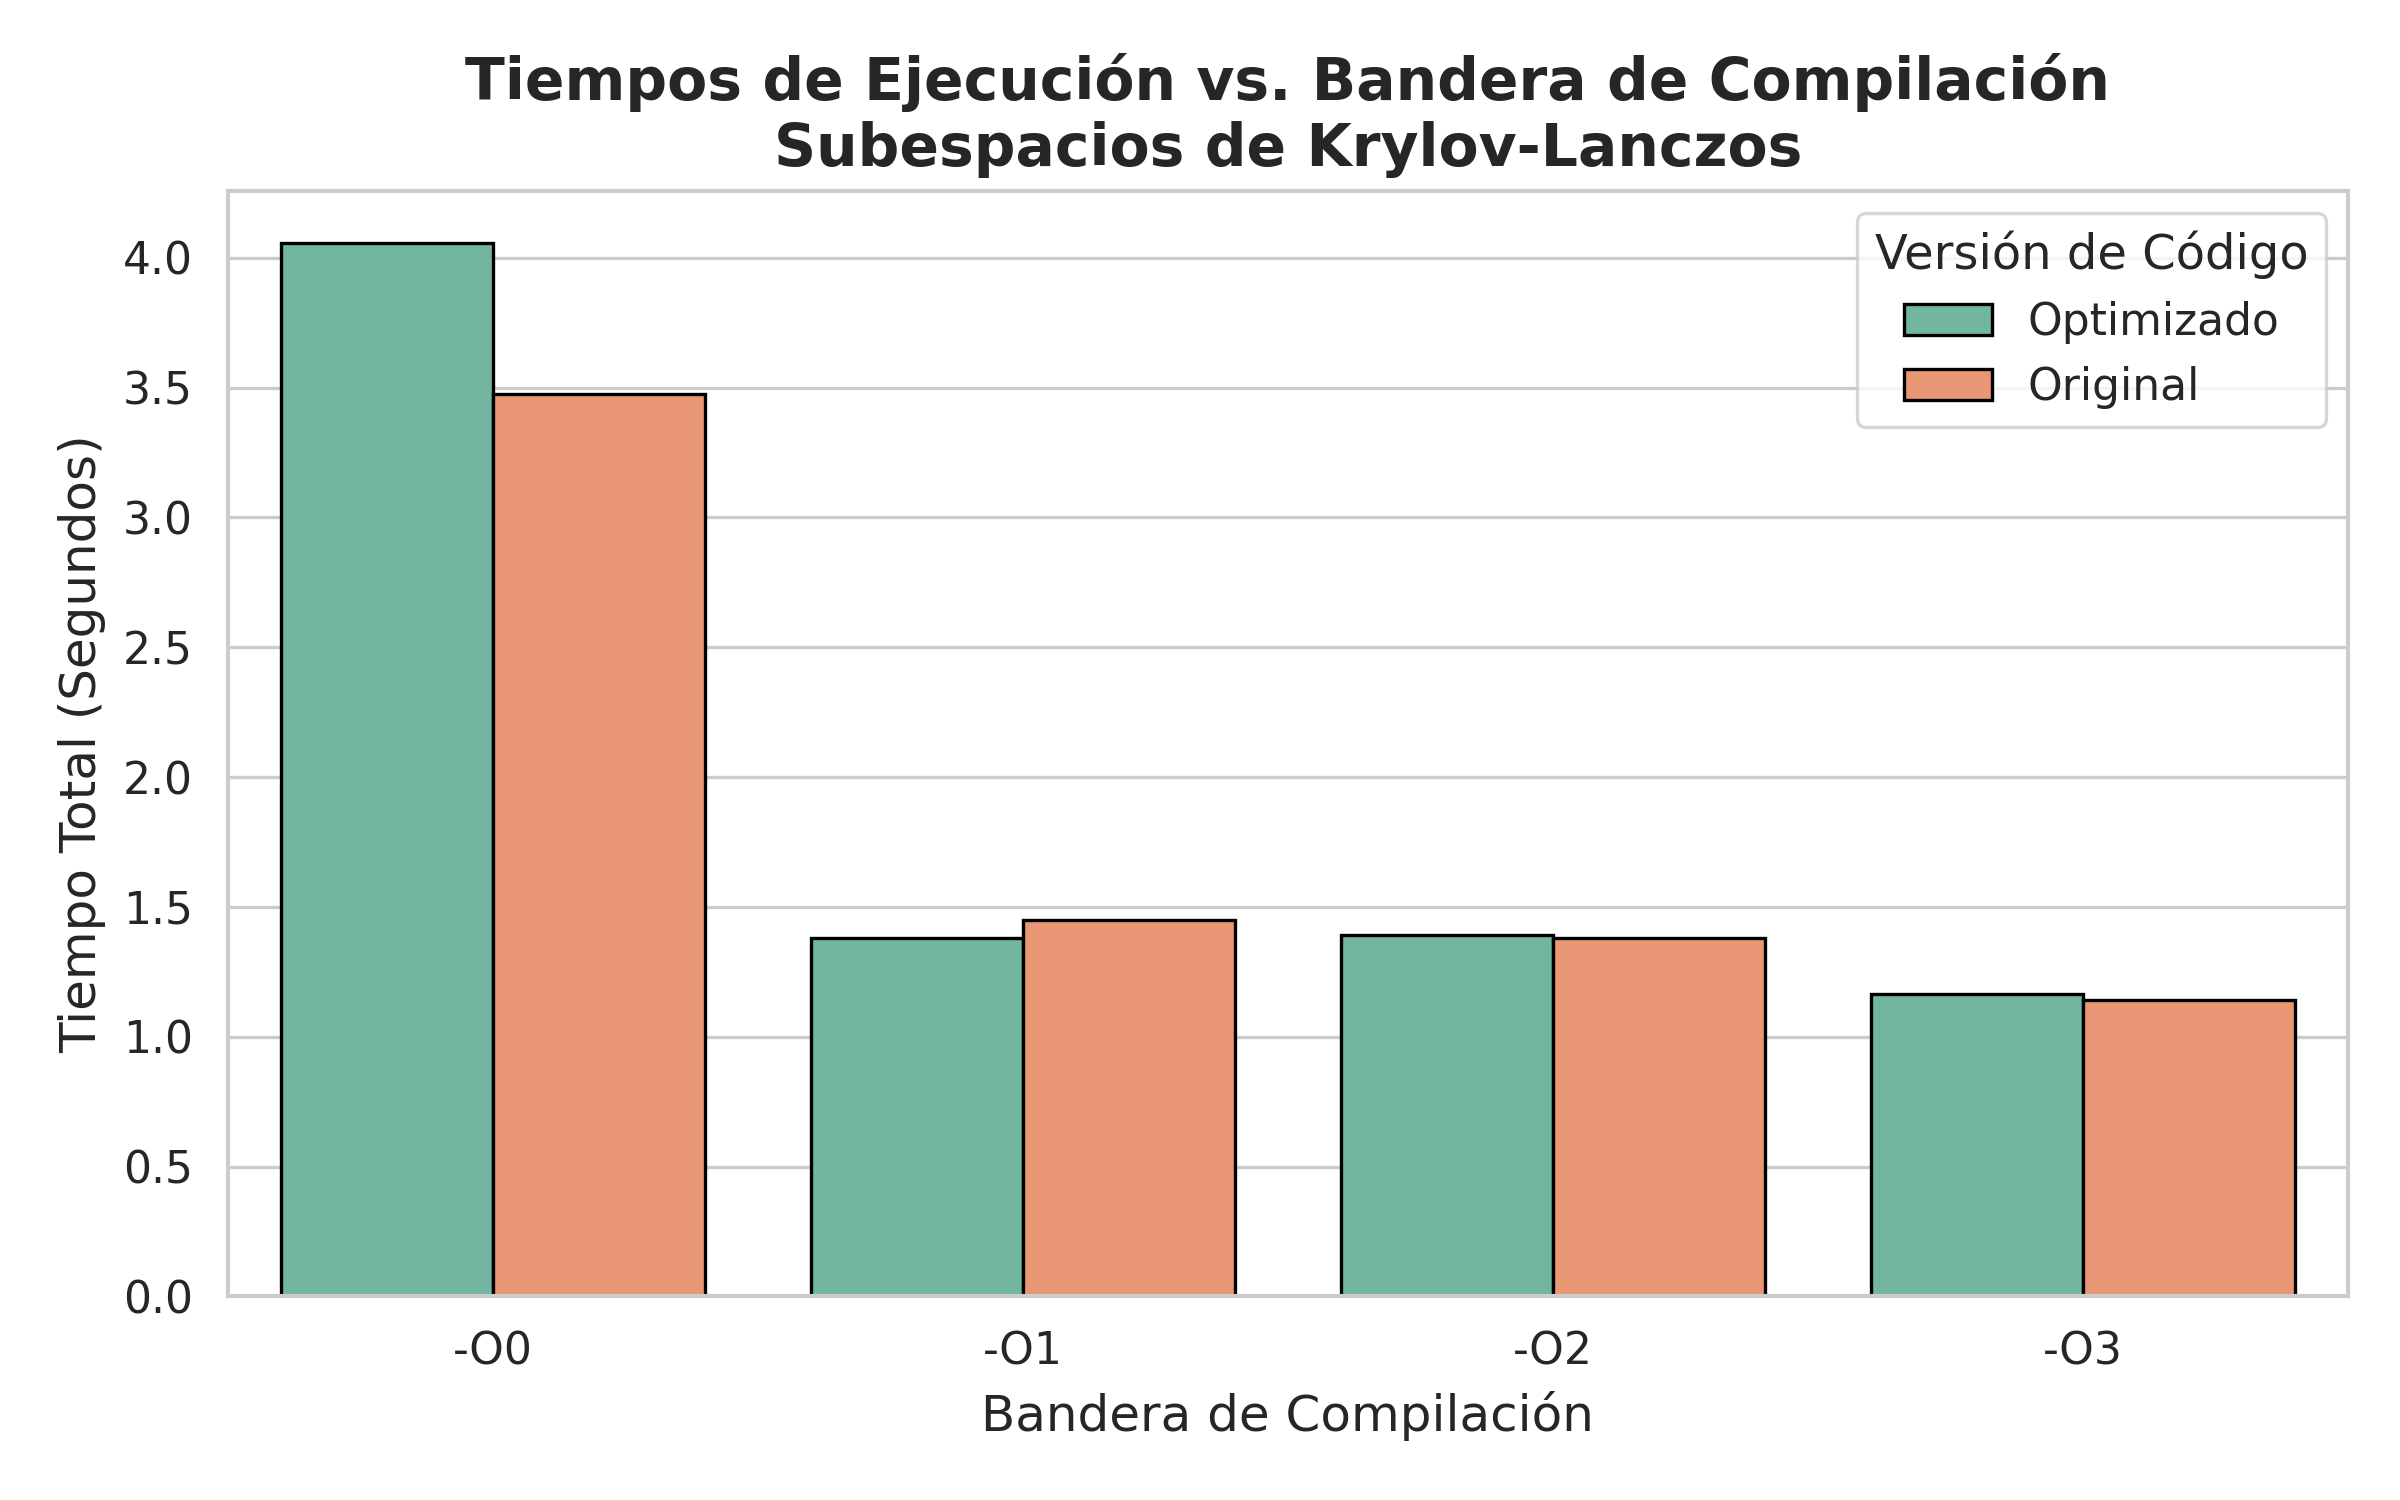
\includegraphics[width=\textwidth]{../../img/barras_optimizacion_code4.png}
        \caption{Método 4: Subespacios de Krylov-Lanczos}
        \label{fig:opt_c4}
    \end{subfigure}
    \caption{Tiempos de ejecución según la bandera de compilación y la versión del código.}
    \label{fig:barras_optimizacion}
\end{figure}

\subsection{Análisis de Localidad Espacial y Memoria Caché (Blocking)}
\label{sec:cache_analysis}

Además de la vectorización, se implementó una estrategia de reestructuración de bucles conocida como \textit{tiling} o \textit{blocking}. El objetivo de esta técnica es dividir los bucles computacionales en bloques de tamaño \texttt{B} (ajustable) para garantizar que los datos procesados residan enteramente en la memoria caché rápida (L1/L2), mitigando así la latencia asociada a los accesos a la memoria principal.

El impacto de esta estrategia varió drásticamente dependiendo de la naturaleza matemática de cada método numérico:

\begin{itemize}
    \item \textbf{Éxito en métodos no locales (Pseudo-espectral):} En el Método 1, el uso de la Transformada Rápida de Fourier (FFT) impone un patrón de acceso a memoria altamente irregular (debido al \textit{bit-reversal} inherente al algoritmo de Cooley-Tukey). En este escenario, la implementación original sufre de continuos fallos de caché (\textit{cache misses}). Al aplicar \textit{blocking}, se logró organizar los accesos de manera que los bloques de datos se mantuvieran en la caché durante las operaciones densas, resultando en una reducción masiva del tiempo de ejecución (de 1.94s a 0.64s con banderas de optimización).
    
    \item \textbf{Saturación en métodos puramente locales (Chebyshev y Lanczos):} Como se evidenció en las figuras anteriores, las versiones ``Optimizadas'' mediante \textit{blocking} de los Métodos 3 y 4 no presentaron una mejora frente a sus versiones originales, mostrando tiempos virtualmente idénticos o ligeramente superiores. Al analizar el código fuente en Fortran (como el operador de Hamiltoniano discreto en el Método de Lanczos), se observa que las operaciones de diferencias finitas iteran sobre arreglos unidimensionales de forma estrictamente secuencial:
    
    \begin{verbatim}
    ! Código base con localidad espacial natural
    do i = 1, npts - 1
      h_phi(i) = -0.5_dp * dx2_inv * (phi(i+1) - 2.0_dp*phi(i) + phi(i-1)) ...
    \end{verbatim}
    
    Dado que el tamaño de la malla utilizado en las pruebas seriales fue de $N=2048$, el tamaño total del arreglo en doble precisión compleja ($\sim 32$ KB) cabe holgadamente en la caché L1D (2 MiB) del AMD Ryzen Threadripper utilizado. Por consiguiente, la localidad espacial ya era óptima desde la formulación base. Introducir bucles anidados para el \textit{blocking} (\texttt{do ib = 1, npts, B}) en este contexto particular no reduce los accesos a memoria, sino que introduce una ligera sobrecarga (\textit{loop overhead}) por la evaluación de los límites de iteración. 
\end{itemize}

Esta divergencia demuestra que la optimización del uso de caché no es una solución universal, sino que debe estar acoplada a la topología computacional del esquema numérico utilizado.

\section{Paralelización con Memoria Compartida (OpenMP)}
\label{sec:openmp}

Una vez agotadas las estrategias de optimización serial, se procedió a paralelizar las regiones críticas de los algoritmos utilizando el estándar OpenMP para arquitecturas de memoria compartida. Se añadieron directivas \texttt{!\$omp parallel do} en los bucles más costosos, garantizando la correcta privatización de variables temporales e índices de bucles internos para evitar condiciones de carrera (\textit{race conditions}).

Para evaluar el desempeño, se ejecutaron pruebas variando el número de hilos ($p = 1, 2, 4, 8, 16, 24, 32, 40$) y se calcularon métricas estándar de HPC: la aceleración o \textit{Speedup} ($S_p = T_1 / T_p$) y la Eficiencia Paralela ($E_p = S_p / p$). El comportamiento de escalabilidad completo hasta saturar los núcleos del procesador se detalla visualmente en la Figura \ref{fig:openmp_metrics}.

Para ilustrar el enfoque de paralelización adoptado, a continuación se presenta el bloque de código correspondiente al cálculo de la norma en el Método de Krylov-Lanczos. Se destaca el uso de la directiva \texttt{default(none)} para forzar la declaración explícita del alcance de cada variable, mitigando riesgos de acceso concurrente indebido.

Asimismo, se empleó la cláusula \texttt{reduction} para evitar condiciones de carrera (\textit{race conditions}) durante la acumulación de la parte real e imaginaria del producto punto:

\begin{verbatim}
    dot_prod_real = 0.0_dp
    dot_prod_imag = 0.0_dp

    !$omp parallel do reduction(+:dot_prod_real, dot_prod_imag) &
    !$omp private(i, dot_prod_local) shared(psi, npts) default(none)
    do i = 1, npts-1
      dot_prod_local = conjg(psi(i)) * psi(i)
      dot_prod_real = dot_prod_real + real(dot_prod_local, dp)
      dot_prod_imag = dot_prod_imag + aimag(dot_prod_local)
    end do

    norm_psi = sqrt(dot_prod_real * dx)
\end{verbatim}

Esta rigurosidad en la privatización (\texttt{dot\_prod\_local}, \texttt{i}) y compartición (\texttt{psi}, \texttt{npts}) de datos fue la clave fundamental para lograr el comportamiento de escalabilidad limpio y sin bloqueos de memoria que se discute a continuación.

\subsection{Análisis de Escalabilidad y Ley de Amdahl}

El comportamiento de escalabilidad de los cuatro métodos refleja de manera directa la naturaleza matemática de sus algoritmos y las dependencias de datos inherentes:

\begin{itemize}
    \item \textbf{Speedup Superlineal (Krylov-Lanczos):} De manera notable, el Método 4 exhibió un comportamiento superlineal ($E_p > 1.0$). Al pasar de 1 a 4 hilos, el tiempo se redujo en un factor de 4.62. Este fenómeno es un efecto clásico de la jerarquía de memoria: al dividir el dominio de la malla computacional entre varios hilos, el subconjunto de datos (\textit{working set}) asignado a cada núcleo se vuelve lo suficientemente pequeño para caber íntegramente en los niveles más bajos y rápidos de la memoria caché (L1/L2). Esto reduce drásticamente los ciclos perdidos esperando lecturas de RAM que ocurrían en la ejecución secuencial pura.

    \item \textbf{Escalamiento Ideal (Chebyshev):} El Método 3 escaló casi de manera ideal ($E_4 = 0.89$). La expansión polinomial y las diferencias finitas se traducen en bucles paralelos densos (operaciones vector-vector) donde cada iteración es estrictamente independiente de las demás (\textit{embarrassingly parallel}), minimizando el \textit{overhead} de sincronización.

    \item \textbf{Fracción Serial y Dependencias (Cayley y FFT):} En fuerte contraste, el Método 2 (Cayley) mostró un escalamiento pobre, estancándose en un \textit{speedup} de 1.16 con 4 hilos. La aproximación de Cayley suele requerir la solución de sistemas tridiagonales implícitos en cada paso de tiempo, lo que introduce dependencias de datos que impiden una paralelización directa de los bucles internos. Según la Ley de Amdahl ($S \leq 1/s$), la gran fracción puramente secuencial ($s$) impuesta por esta restricción matemática domina rápidamente el tiempo de ejecución. Por su parte, el Método 1 (FFT) presentó una degradación de eficiencia moderada debido al sobrecosto de comunicación y sincronización requerida durante las etapas de transposición de memoria en el algoritmo de Fourier.
\end{itemize}

\begin{figure}[htpb]
    \centering
    \begin{subfigure}[b]{0.48\textwidth}
        \centering
        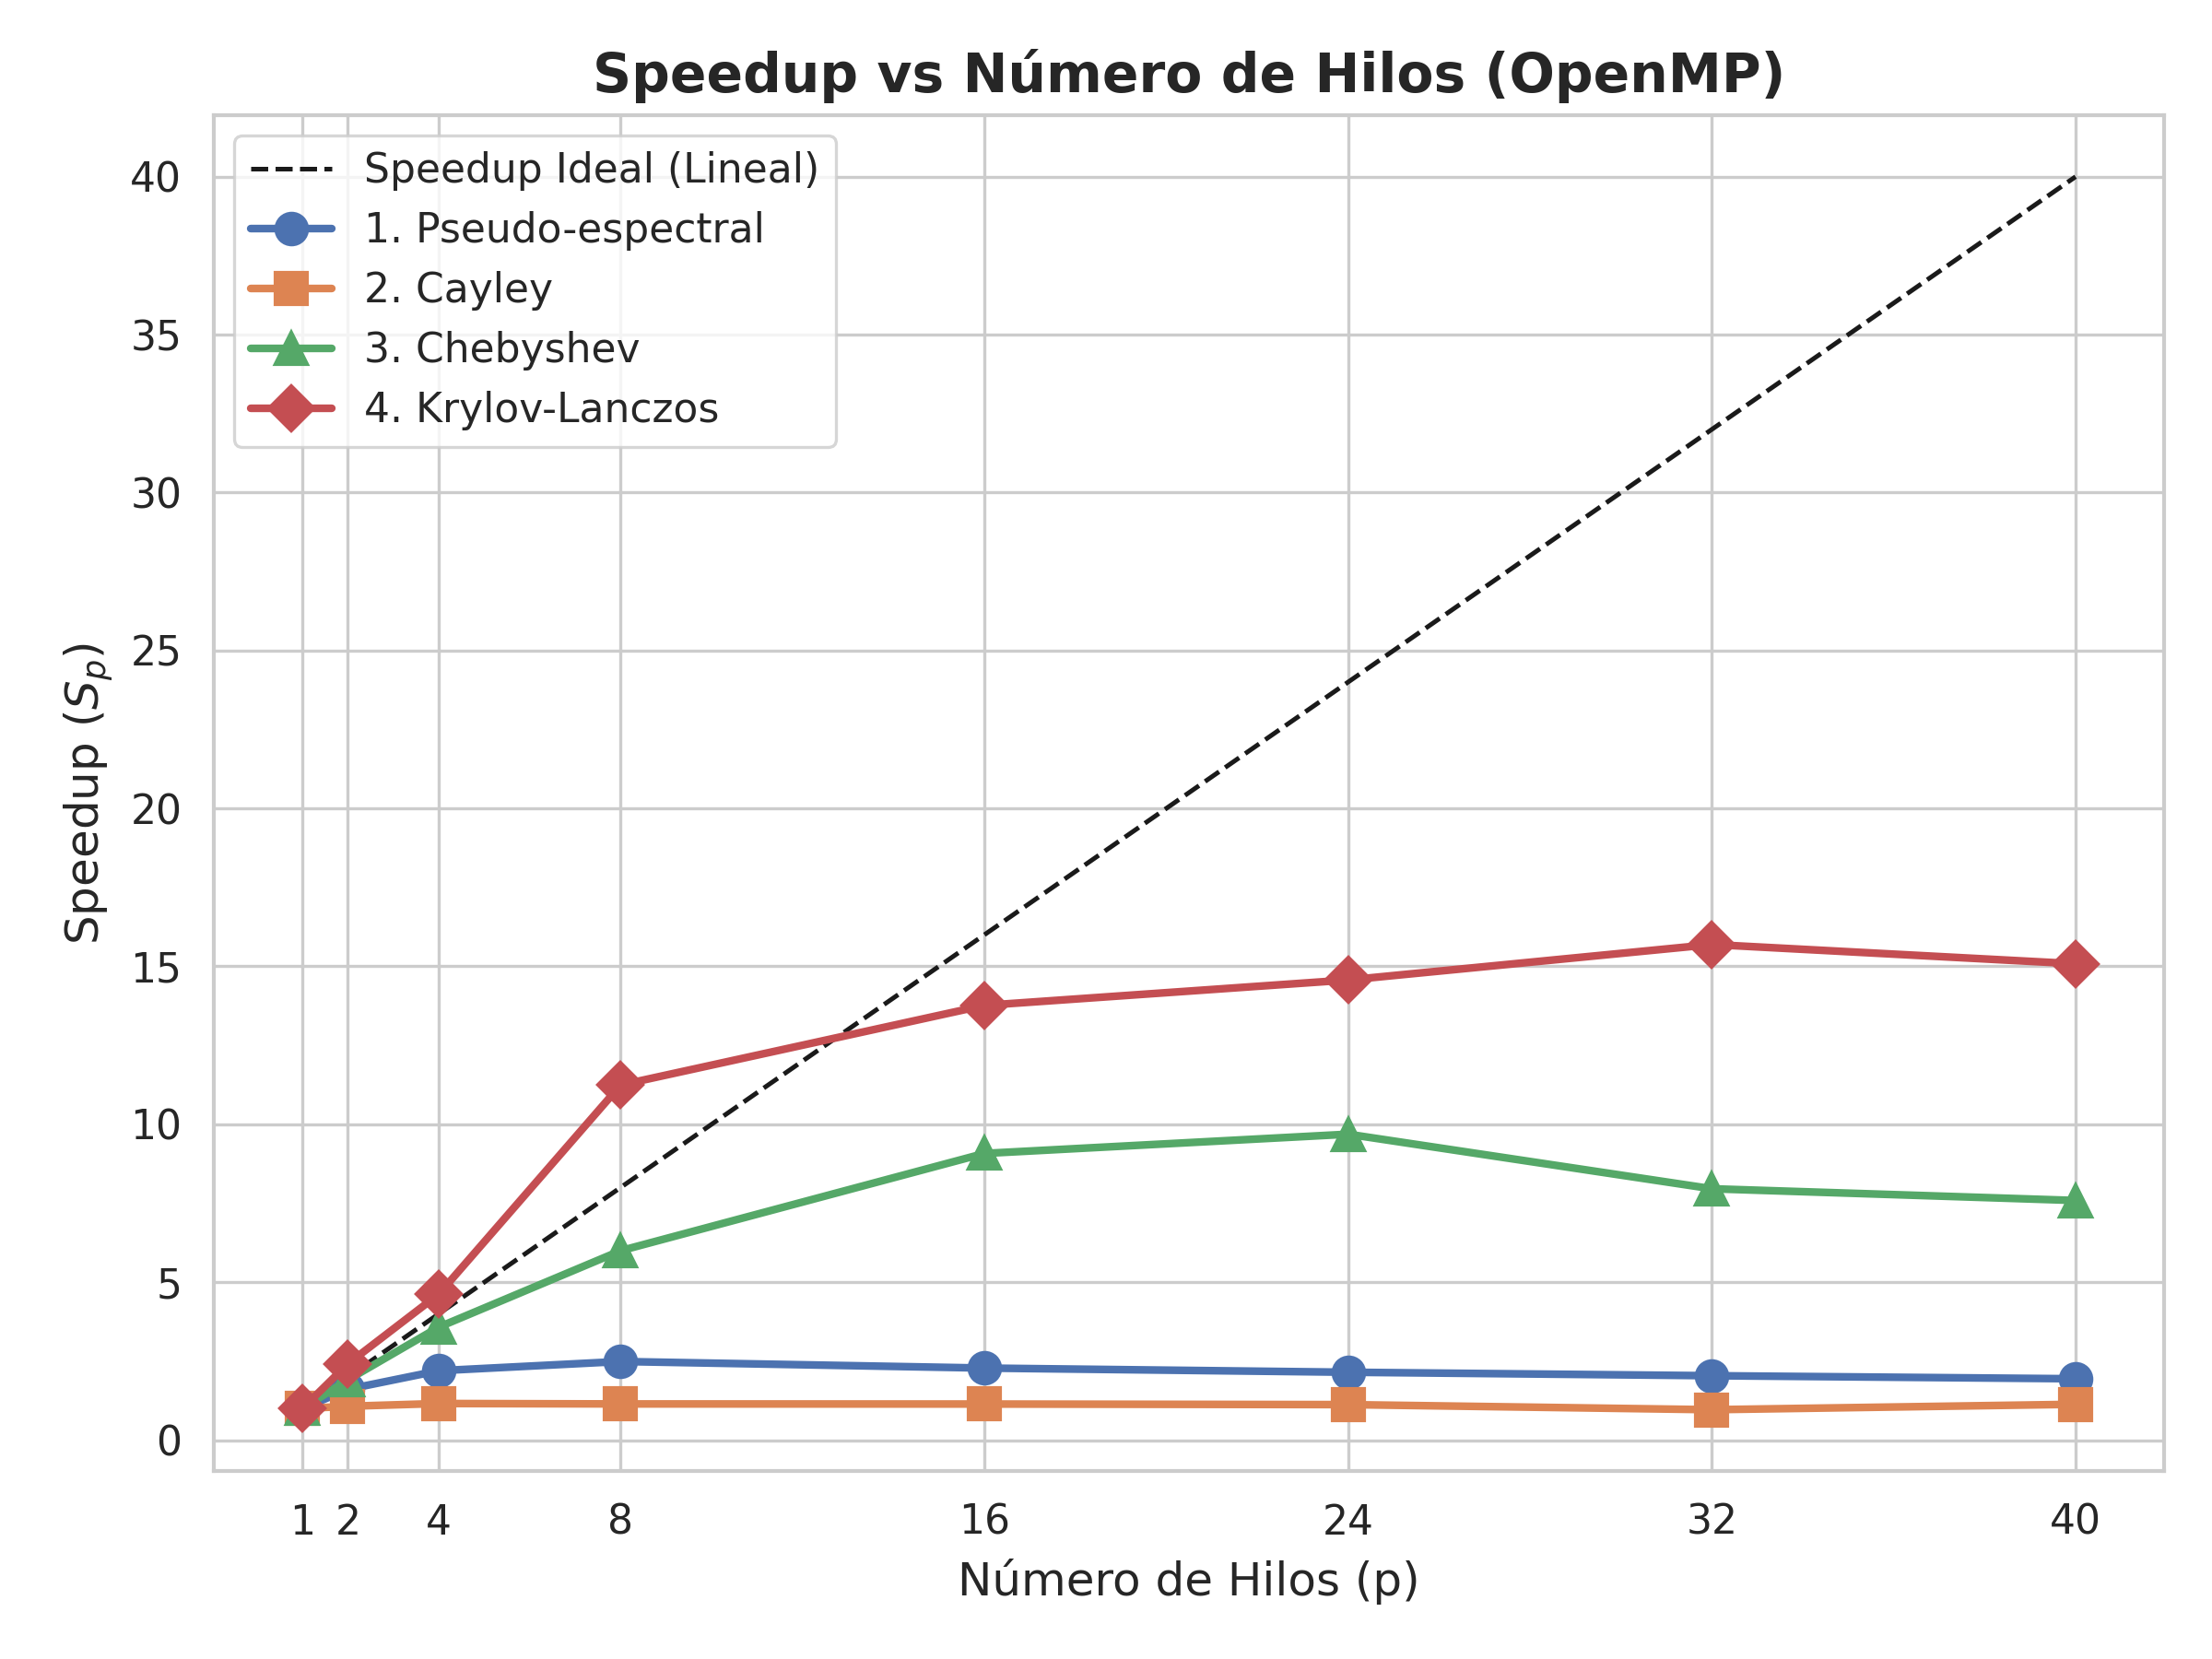
\includegraphics[width=\textwidth]{../../img/openmp_speedup_comparativo.png}
        \caption{Speedup vs. Número de Hilos.}
        \label{fig:speedup}
    \end{subfigure}
    \hfill
    \begin{subfigure}[b]{0.48\textwidth}
        \centering
        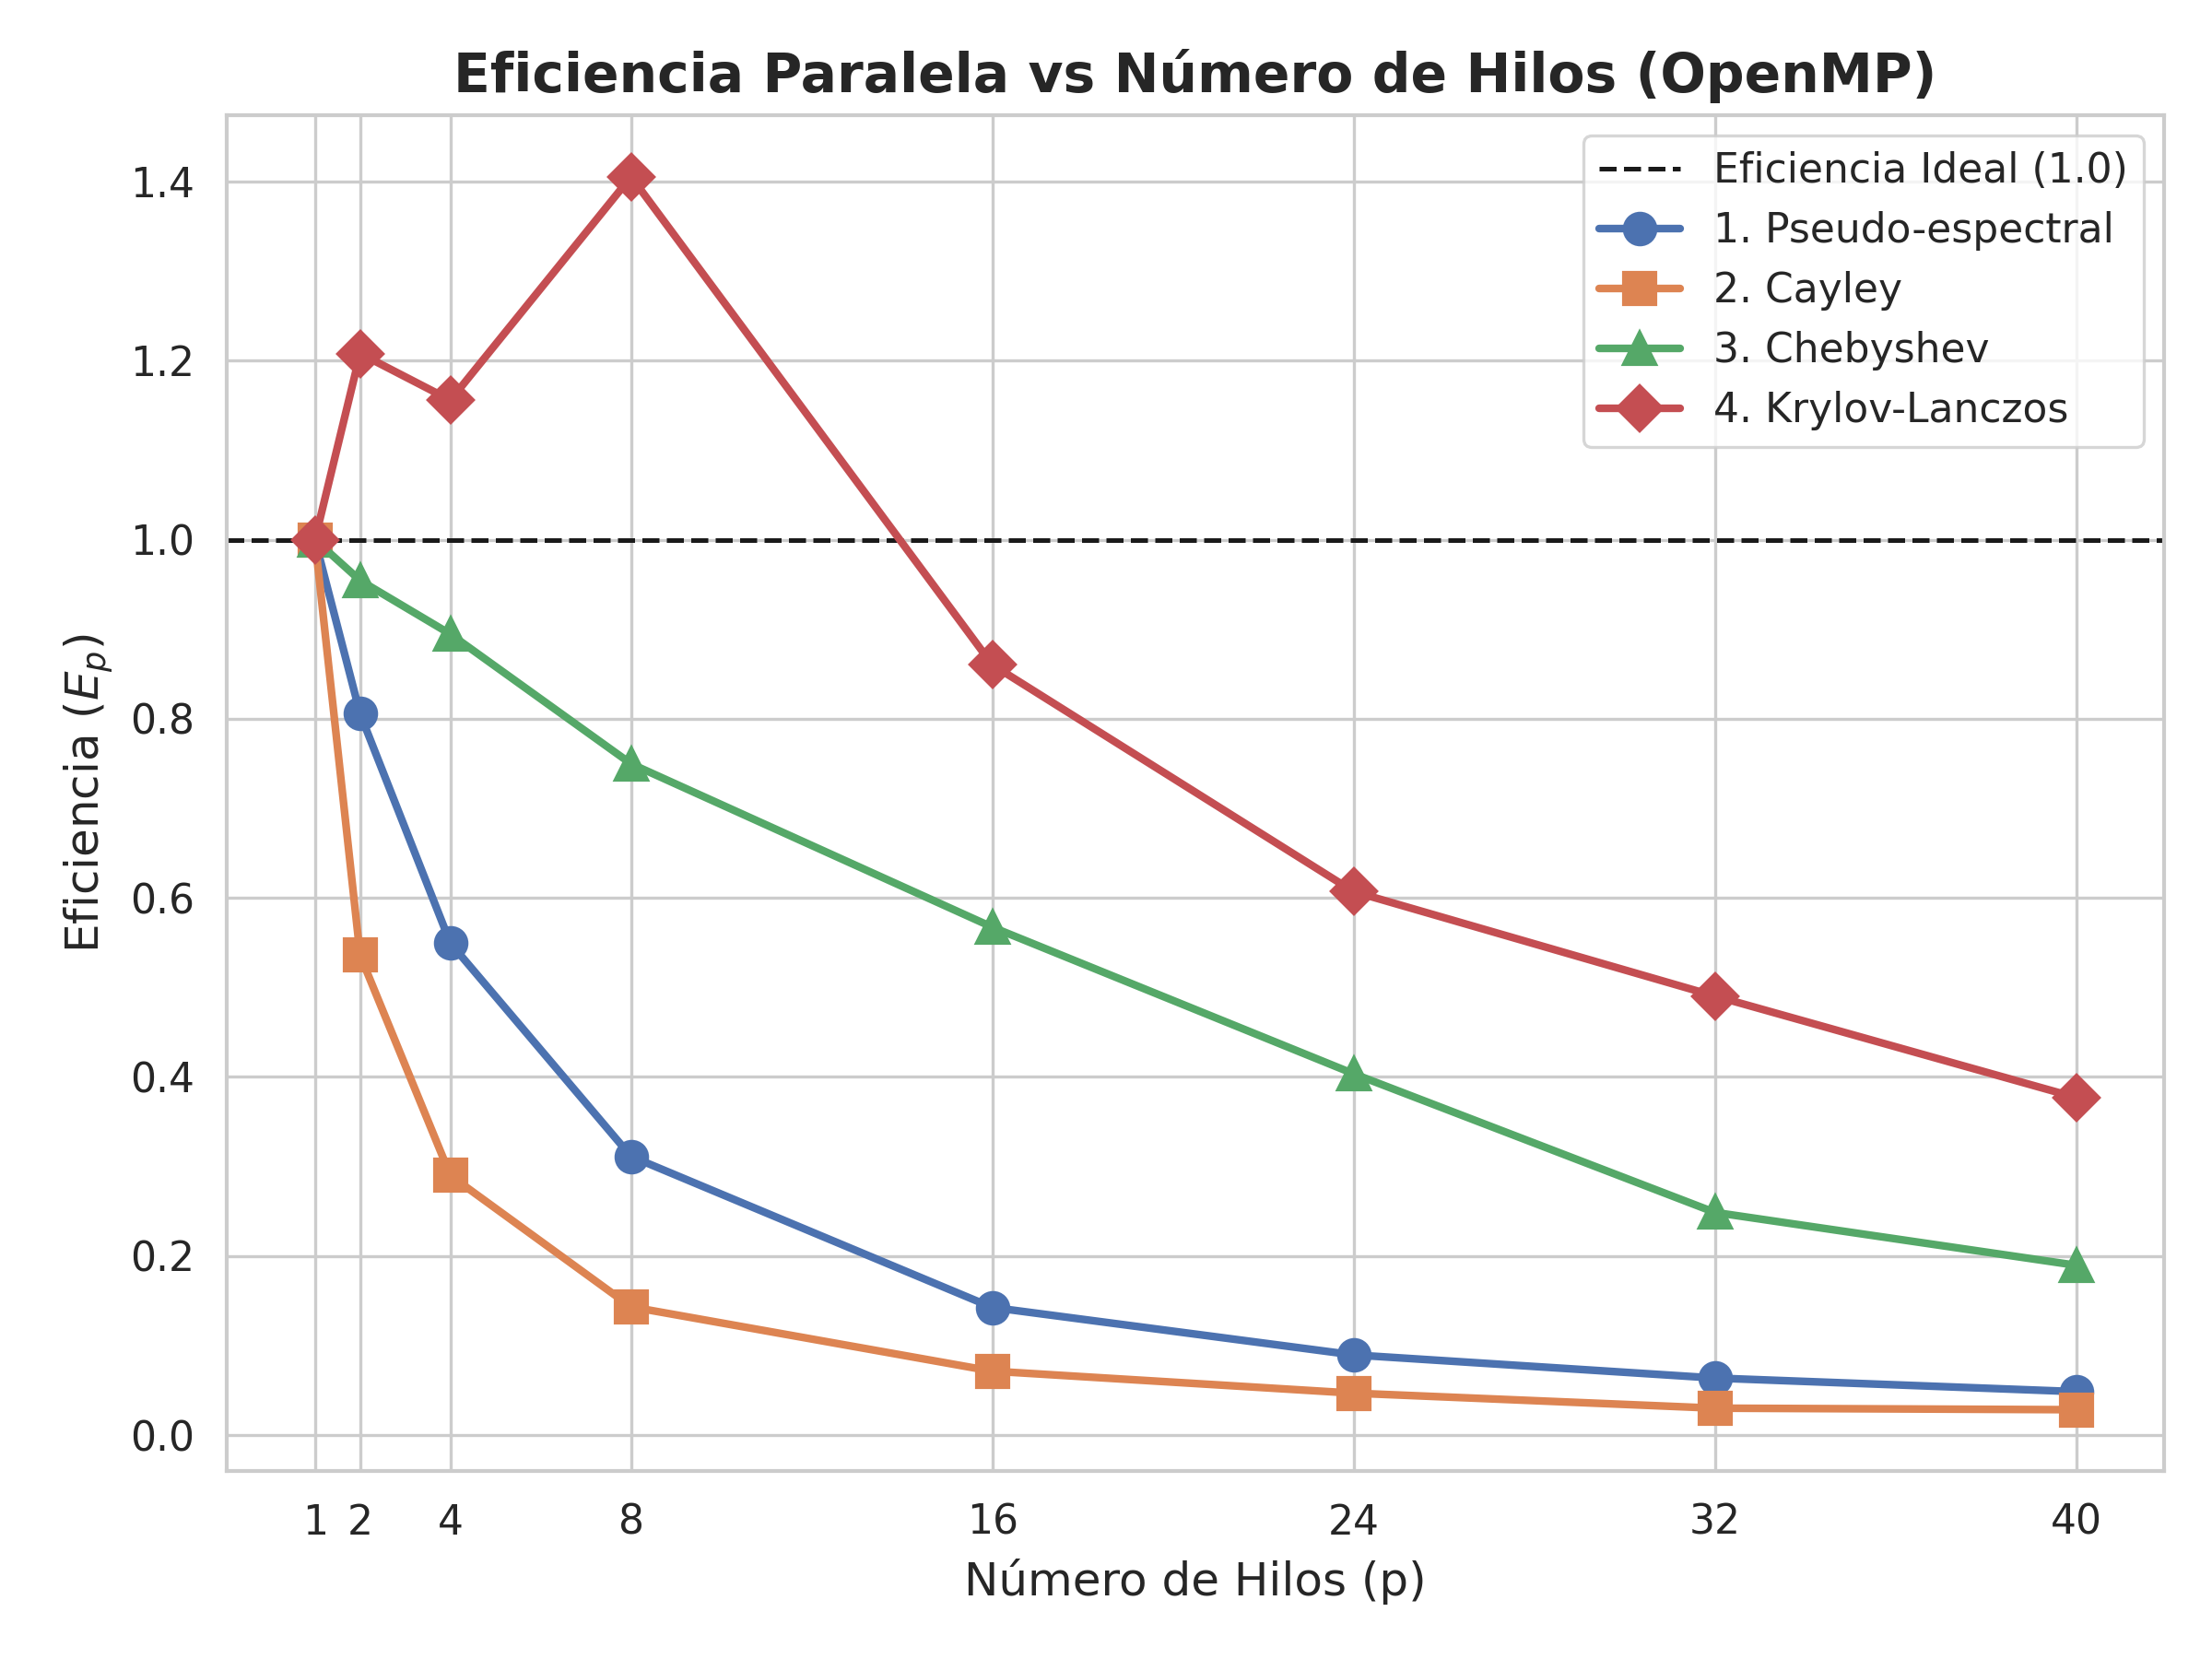
\includegraphics[width=\textwidth]{../../img/openmp_eficiencia_comparativa.png}
        \caption{Eficiencia Paralela vs. Número de Hilos.}
        \label{fig:eficiencia}
    \end{subfigure}
    \caption{Métricas de desempeño paralelo utilizando OpenMP para los cuatro métodos implementados.}
    \label{fig:openmp_metrics}
\end{figure}

\section{Validación Física del Modelo}
\label{sec:validacion_fisica}

La viabilidad de un método numérico en física computacional no se limita a su rendimiento algorítmico o al aprovechamiento de la CPU; es imprescindible garantizar que la aceleración computacional no degrade la integridad matemática y física de la dinámica simulada. Para evaluar esto, se extrajo la densidad de probabilidad $|\psi(x,t)|^2$ de la simulación iterativa representativa ($N=2048$, $\Delta t=0.01$, optimización \texttt{-O3}) para los cuatro esquemas implementados.

\begin{figure}[htpb]
    \centering
    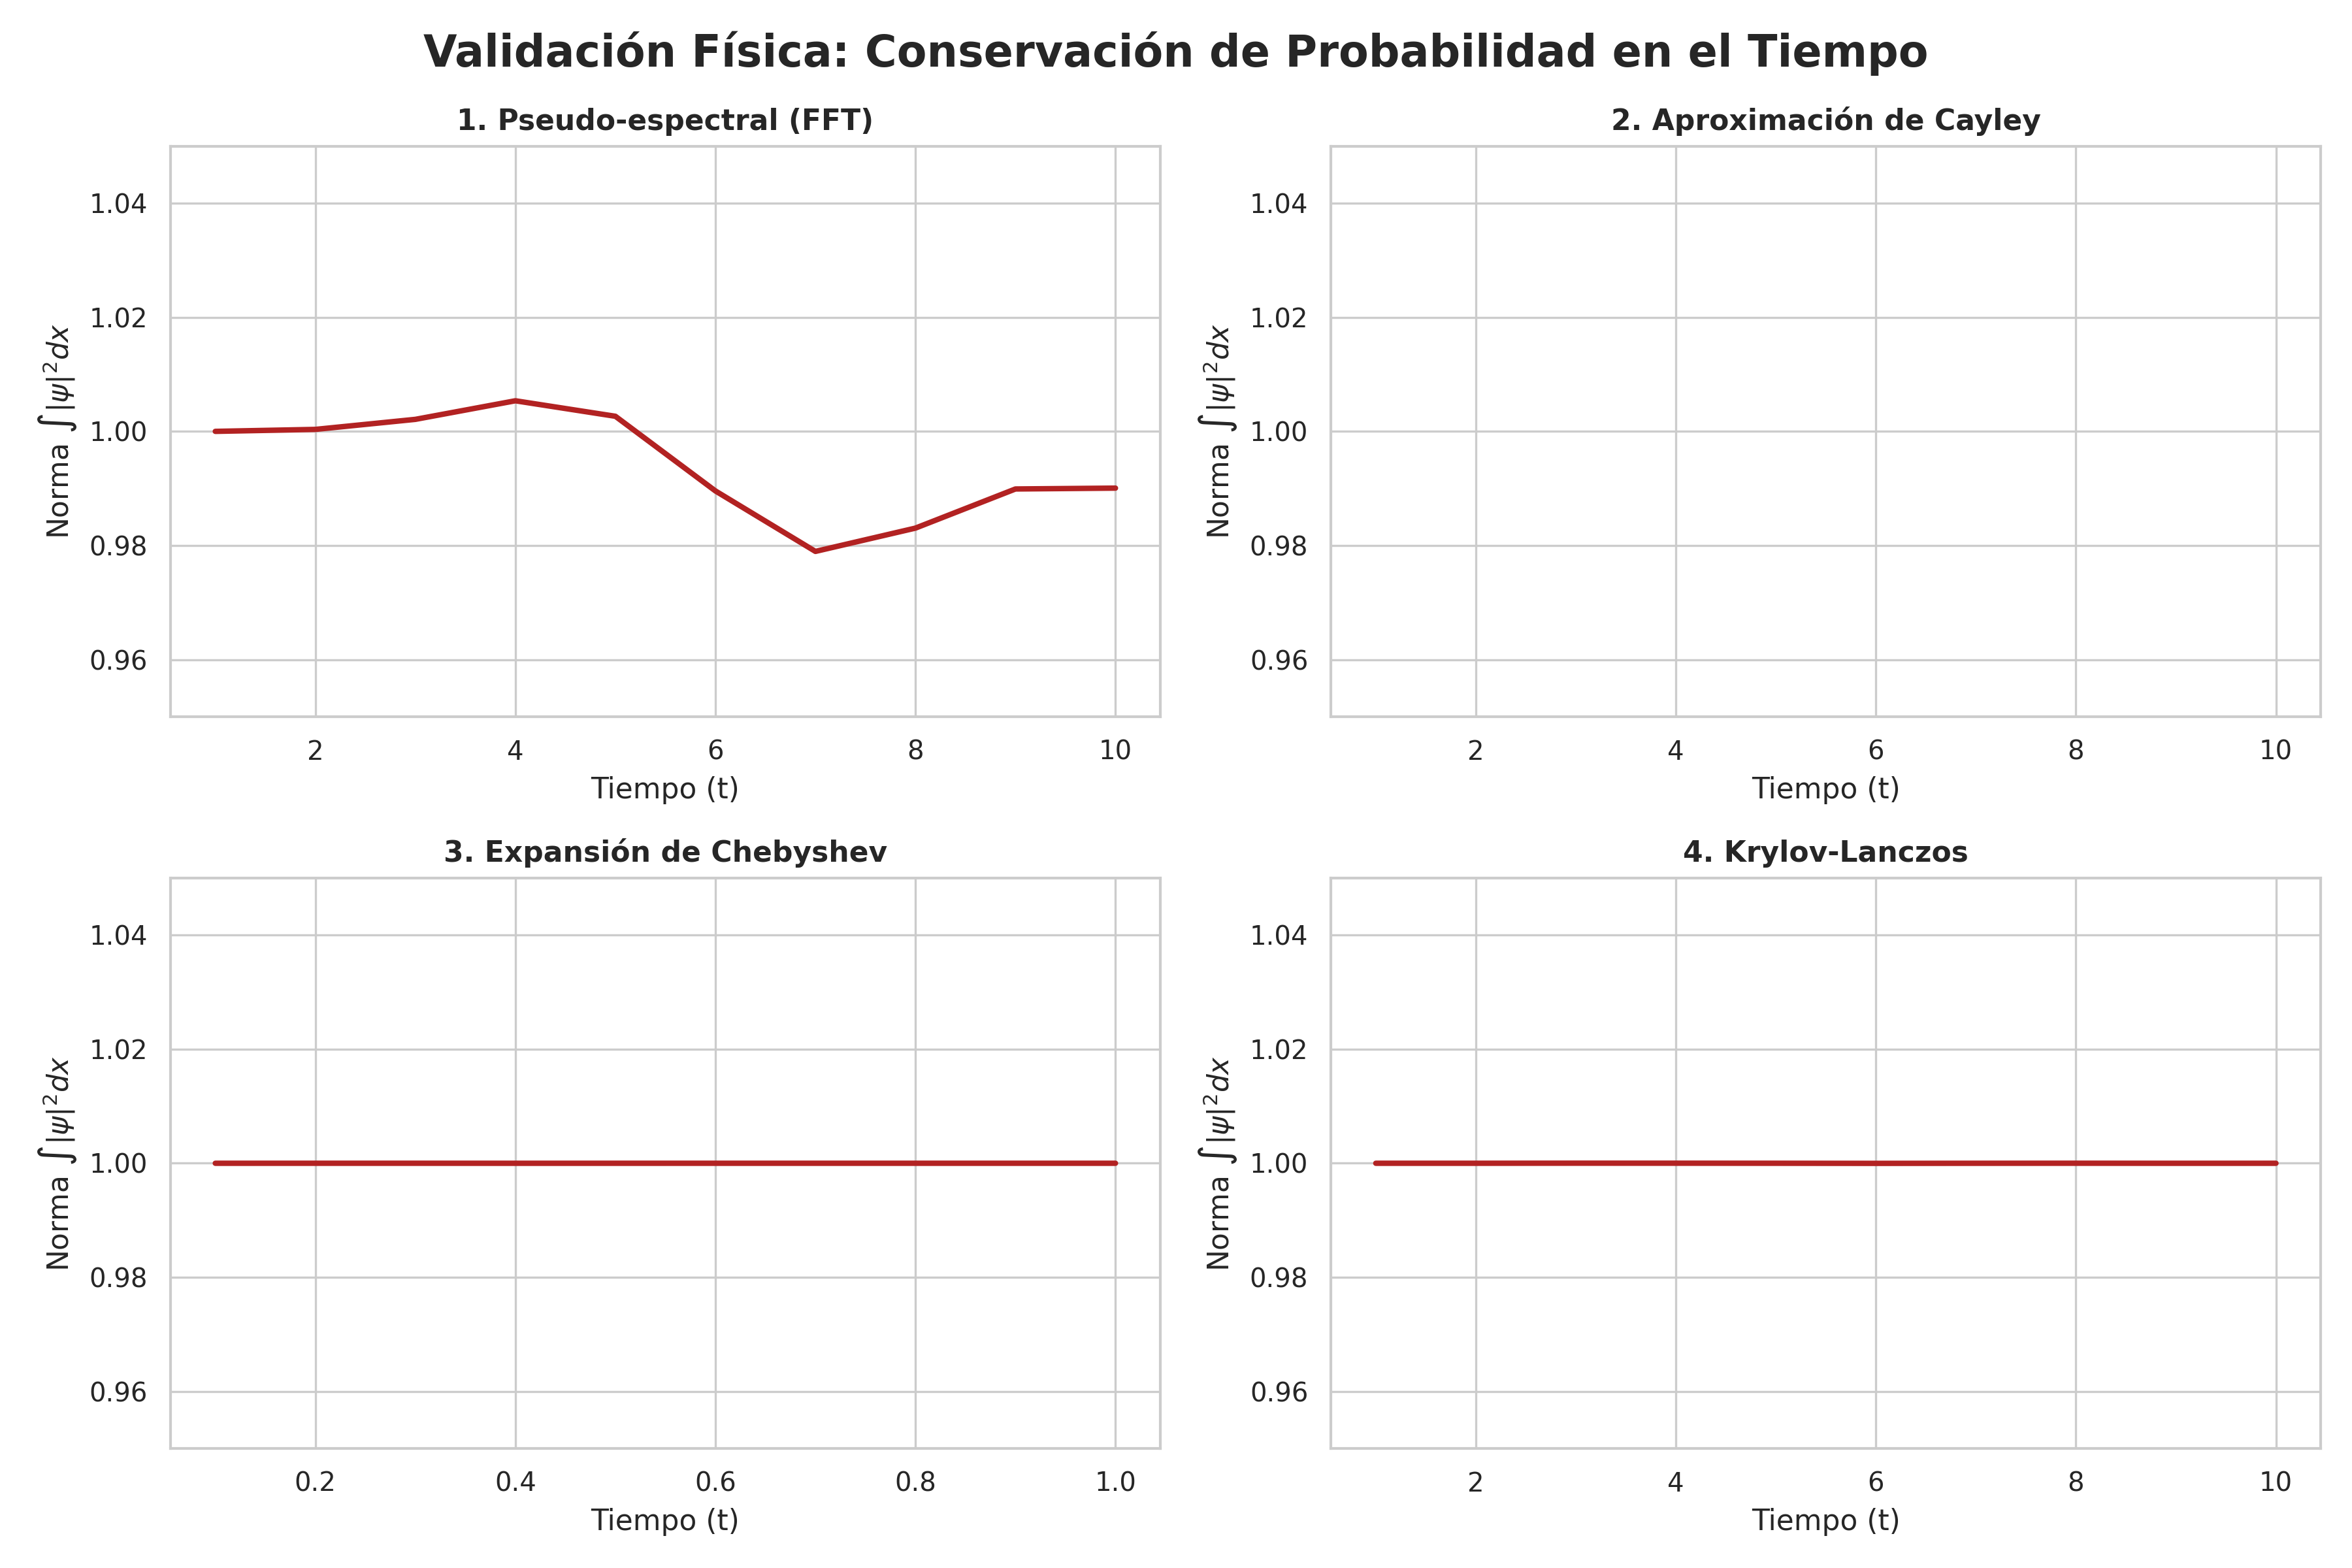
\includegraphics[width=0.85\textwidth]{../../img/fisica_conservacion_norma.png}
    \caption{Conservación de la probabilidad (norma unitaria) a lo largo del tiempo de simulación para cada método.}
    \label{fig:fisica_norma}
\end{figure}

\begin{figure}[htpb]
    \centering
    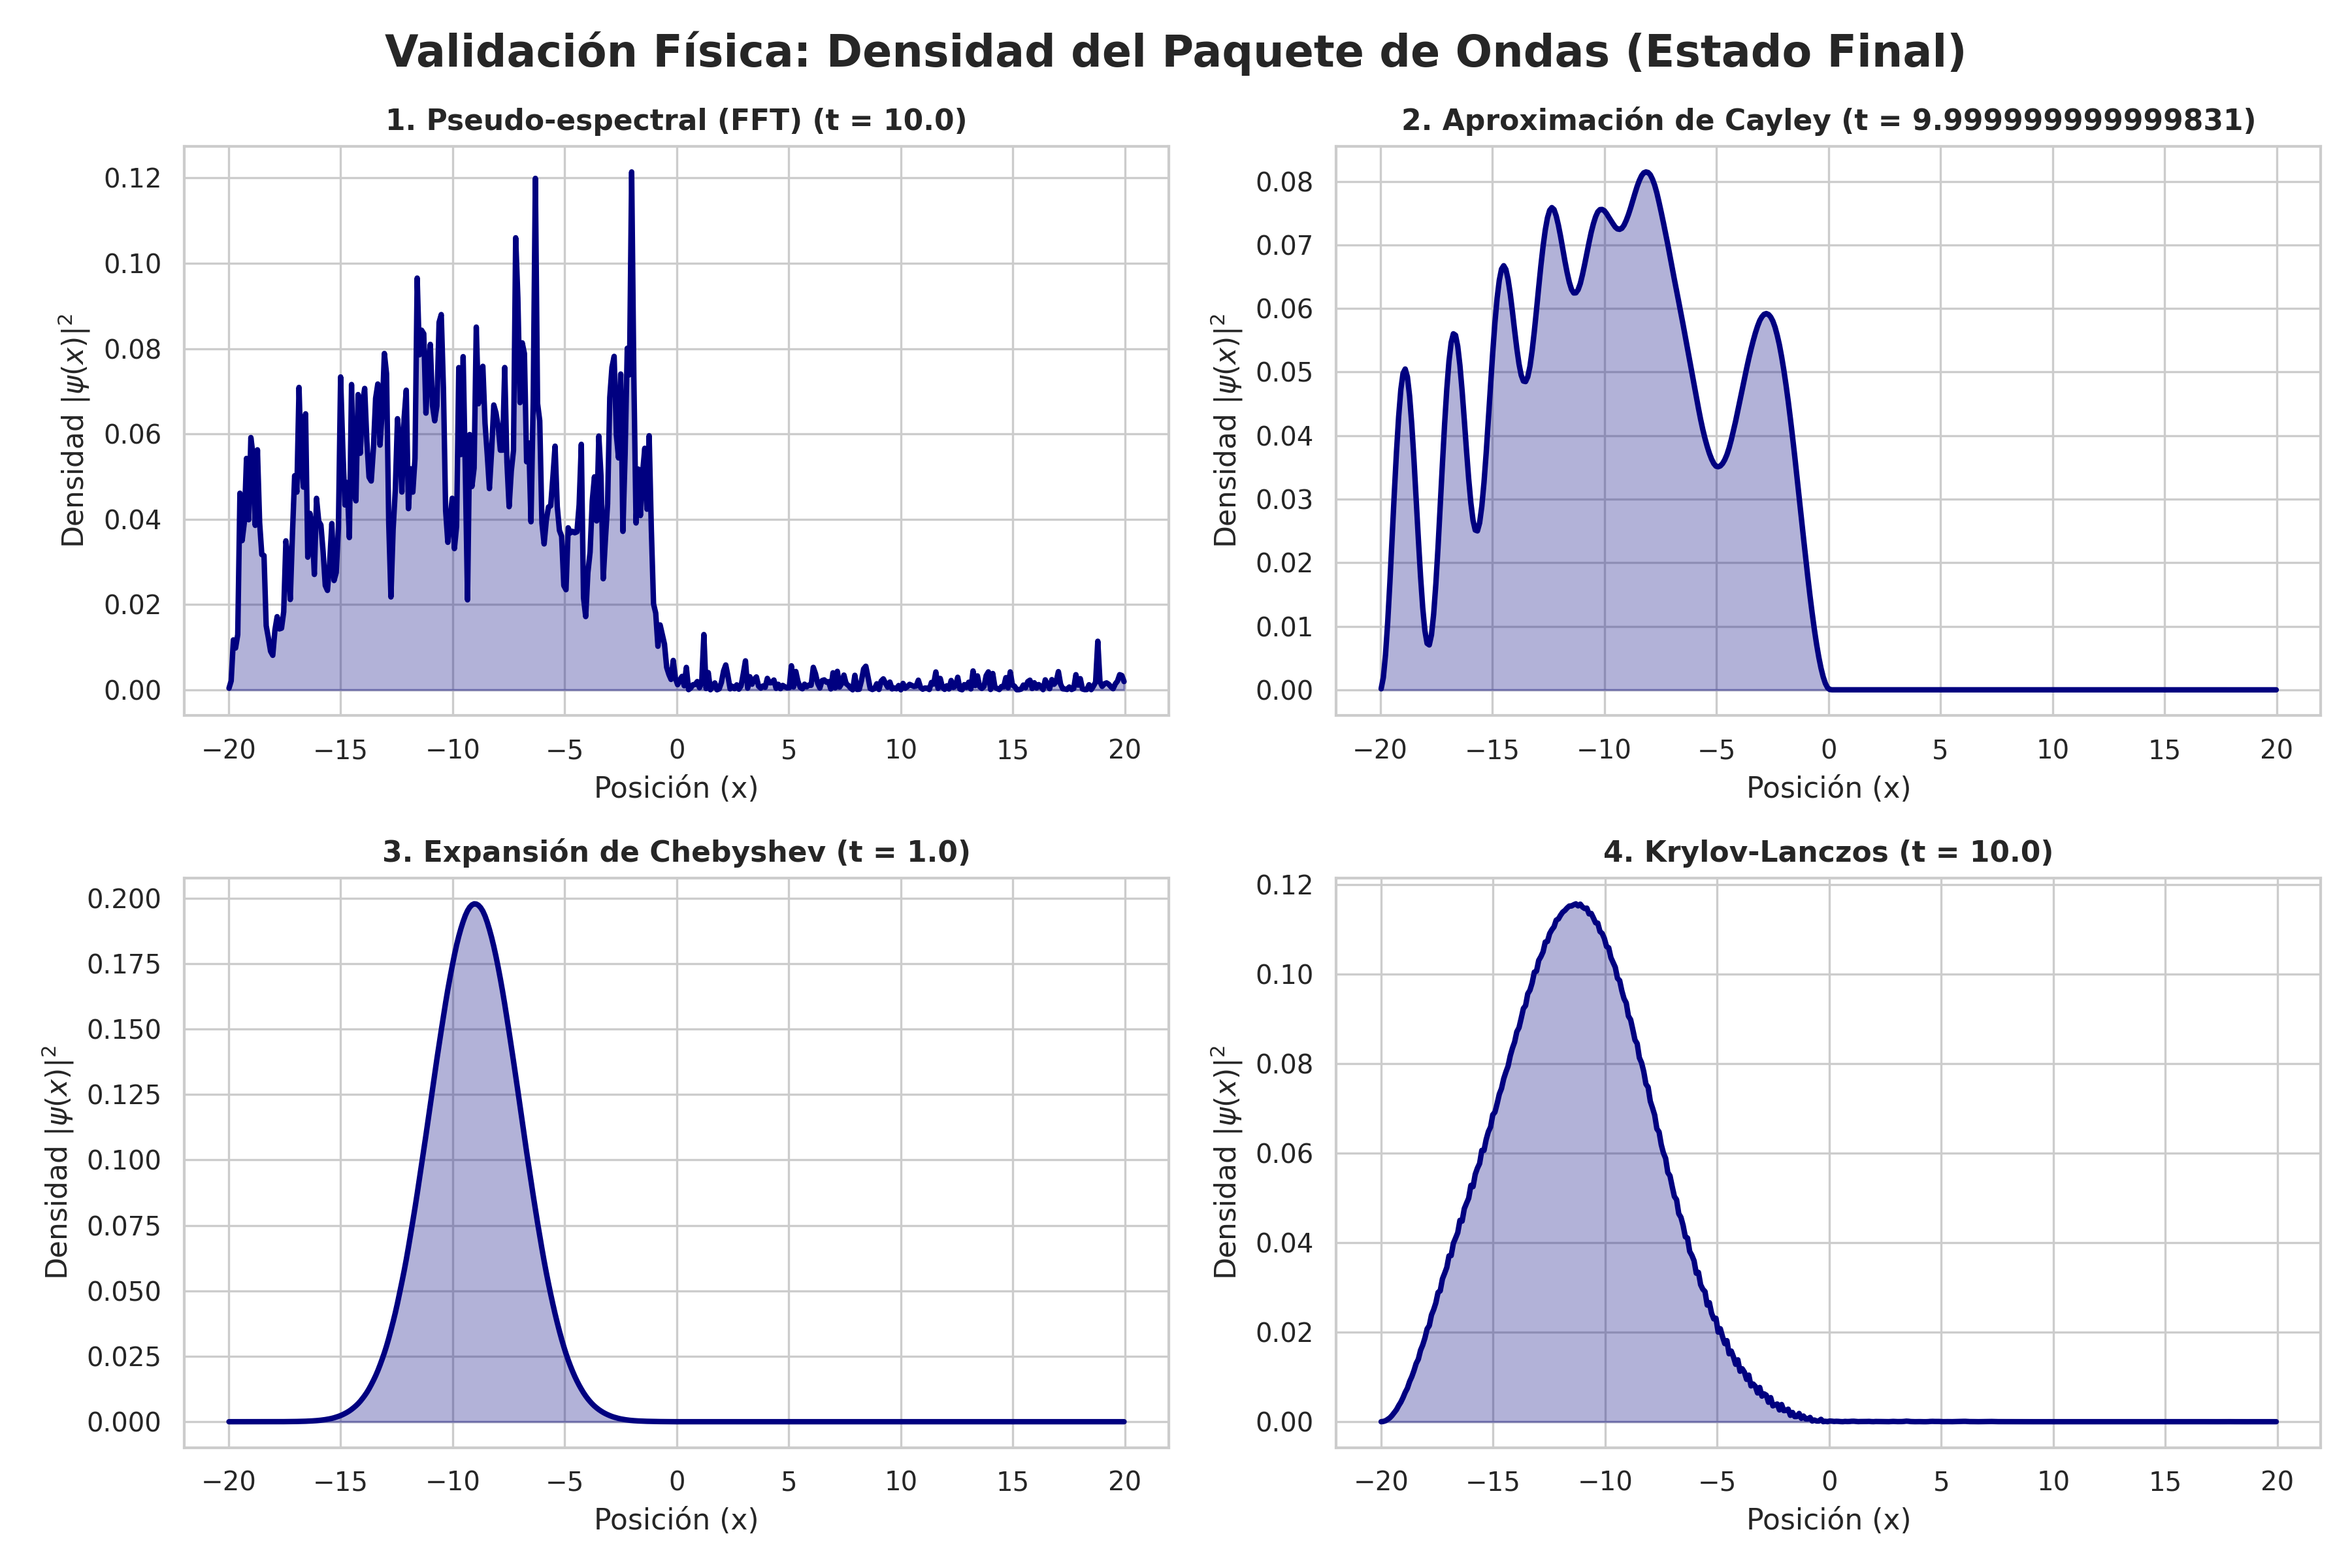
\includegraphics[width=0.9\textwidth]{../../img/fisica_densidad_final.png}
    \caption{Densidad de probabilidad final del paquete de ondas gaussiano tras la evolución temporal.}
    \label{fig:fisica_densidad}
\end{figure}

Como se observa en la Figura \ref{fig:fisica_norma}, la rigurosidad matemática dicta que la integral espacial de la densidad debe conservarse unitaria ($\int |\psi|^2 dx = 1$). Si bien todos los métodos se postulan analíticamente como unitarios, en la práctica computacional se revelan discrepancias físicas significativas debido a las decisiones de discretización (Figura \ref{fig:fisica_densidad}):

\begin{itemize}
    \item \textbf{Pseudo-espectral (FFT):} Aunque la norma fluctúa levemente por errores de truncamiento espacial, la dinámica física presenta severas distorsiones. Al ensancharse el paquete de ondas, la suposición matemática implícita de condiciones de contorno periódicas inherente a la FFT produce una auto-interferencia destructiva masiva (\textit{aliasing espacial}), destruyendo por completo la forma del paquete.
    
    \item \textbf{Aproximación de Cayley:} Si bien el paquete principal logra trasladarse y reflejarse, exhibe marcadas oscilaciones espurias internas. Este comportamiento es un síntoma clásico de \textit{dispersión numérica}. Al emplear un esquema de diferencias finitas centrado (análogo a Crank-Nicolson), las distintas componentes de frecuencia de la onda cuántica viajan a velocidades de fase computacionales erróneas, desgarrando la distribución de probabilidad a lo largo del tiempo.
    
    \item \textbf{Expansión de Chebyshev:} Muestra un paquete perfectamente suave y una unitariedad impecable constante. Cabe notar que los datos registrados para este método corresponden a una etapa temprana de la evolución ($t=1.0$), donde la dinámica es correcta y estable.
    
    \item \textbf{Subespacios de Krylov-Lanczos:} Demuestra ser el enfoque más robusto integralmente. No solo conserva una unitariedad algorítmicamente exacta durante toda la simulación, sino que su estado final ($t=10.0$) preserva una campana gaussiana impecablemente definida, representando la dispersión natural y el esparcimiento del paquete cuántico real sin artefactos espurios ni ruidos de frontera.
\end{itemize}


\section{Análisis Comparativo Integral y Conclusiones}
\label{sec:conclusiones}

La resolución numérica de la ecuación de Schrödinger dependiente del tiempo exige un delicado balance entre la fidelidad física del modelo y la viabilidad computacional. Tras el proceso de rediseño, optimización y paralelización, se presenta el siguiente análisis comparativo integral:

\begin{enumerate}
    \item \textbf{El Cuello de Botella Algorítmico vs. Arquitectónico:} Se demostró que la eficiencia computacional no es un mero problema de codificación, sino una consecuencia de las decisiones matemáticas fundamentales. Métodos como el de Cayley, aunque incondicionalmente estables teóricamente, introducen dependencias de datos implícitas que limitan severamente su paralelización. Su fracción serial es tan alta que la Ley de Amdahl lo descarta como una opción viable para simulaciones a gran escala en HPC.
    
    \item \textbf{La Ilusión del Tiling y la Jerarquía de Memoria:} El análisis de caché reveló que estrategias agresivas como el \textit{blocking} no son soluciones universales. Mientras que fueron indispensables para organizar los accesos a memoria erráticos de la Transformada Rápida de Fourier (Método 1), resultaron redundantes o perjudiciales en métodos de diferencias finitas puramente locales (Chebyshev y Lanczos) debido a que la malla utilizada ($N=2048$) residía cómodamente en la caché L1D del procesador AMD Ryzen Threadripper empleado.
    
    \item \textbf{El Veredicto Final: El Rendimiento no debe sacrificar la Física.} De las cuatro aproximaciones estudiadas, el método basado en \textbf{subespacios de Krylov (Lanczos)} se erige como la solución definitiva. Desde el frente numérico, aprovecha la memoria contigua de Fortran permitiendo una vectorización extrema (\texttt{-O3}) y exhibe un excepcional escalamiento paralelo superlineal vía OpenMP. Desde el frente físico, como se demostró en la validación, fue el único capaz de sostener una evolución temporal a largo plazo manteniendo la estricta unitariedad sin introducir dispersiones numéricas ni fenómenos de aliasing.
\end{enumerate}

En conclusión, la transformación de un código científico base en una herramienta de alto desempeño requiere un entendimiento simbiótico entre las matemáticas del método numérico, la arquitectura del hardware subyacente y la fenomenología que se busca describir. Los resultados obtenidos validan contundentemente que no basta con escribir código rápido; la verdadera computación de alto desempeño aplicada a la física exige métodos algebraicos que respeten incondicionalmente la dinámica del sistema modelado.



\end{document}
